\documentclass[1p]{elsarticle_modified}
%\bibliographystyle{elsarticle-num}

%\usepackage[colorlinks]{hyperref}
%\usepackage{abbrmath_seonhwa} %\Abb, \Ascr, \Acal ,\Abf, \Afrak
\usepackage{amsfonts}
\usepackage{amssymb}
\usepackage{amsmath}
\usepackage{amsthm}
\usepackage{scalefnt}
\usepackage{amsbsy}
\usepackage{kotex}
\usepackage{caption}
\usepackage{subfig}
\usepackage{color}
\usepackage{graphicx}
\usepackage{xcolor} %% white, black, red, green, blue, cyan, magenta, yellow
\usepackage{float}
\usepackage{setspace}
\usepackage{hyperref}

\usepackage{tikz}
\usetikzlibrary{arrows}

\usepackage{multirow}
\usepackage{array} % fixed length table
\usepackage{hhline}

%%%%%%%%%%%%%%%%%%%%%
\makeatletter
\renewcommand*\env@matrix[1][\arraystretch]{%
	\edef\arraystretch{#1}%
	\hskip -\arraycolsep
	\let\@ifnextchar\new@ifnextchar
	\array{*\c@MaxMatrixCols c}}
\makeatother %https://tex.stackexchange.com/questions/14071/how-can-i-increase-the-line-spacing-in-a-matrix
%%%%%%%%%%%%%%%

\usepackage[normalem]{ulem}

\newcommand{\msout}[1]{\ifmmode\text{\sout{\ensuremath{#1}}}\else\sout{#1}\fi}
%SOURCE: \msout is \stkout macro in https://tex.stackexchange.com/questions/20609/strikeout-in-math-mode

\newcommand{\cancel}[1]{
	\ifmmode
	{\color{red}\msout{#1}}
	\else
	{\color{red}\sout{#1}}
	\fi
}

\newcommand{\add}[1]{
	{\color{blue}\uwave{#1}}
}

\newcommand{\replace}[2]{
	\ifmmode
	{\color{red}\msout{#1}}{\color{blue}\uwave{#2}}
	\else
	{\color{red}\sout{#1}}{\color{blue}\uwave{#2}}
	\fi
}

\newcommand{\Sol}{\mathcal{S}} %segment
\newcommand{\D}{D} %diagram
\newcommand{\A}{\mathcal{A}} %arc


%%%%%%%%%%%%%%%%%%%%%%%%%%%%%5 test

\def\sl{\operatorname{\textup{SL}}(2,\Cbb)}
\def\psl{\operatorname{\textup{PSL}}(2,\Cbb)}
\def\quan{\mkern 1mu \triangleright \mkern 1mu}

\theoremstyle{definition}
\newtheorem{thm}{Theorem}[section]
\newtheorem{prop}[thm]{Proposition}
\newtheorem{lem}[thm]{Lemma}
\newtheorem{ques}[thm]{Question}
\newtheorem{cor}[thm]{Corollary}
\newtheorem{defn}[thm]{Definition}
\newtheorem{exam}[thm]{Example}
\newtheorem{rmk}[thm]{Remark}
\newtheorem{alg}[thm]{Algorithm}

\newcommand{\I}{\sqrt{-1}}
\begin{document}

%\begin{frontmatter}
%
%\title{Boundary parabolic representations of knots up to 8 crossings}
%
%%% Group authors per affiliation:
%\author{Yunhi Cho} 
%\address{Department of Mathematics, University of Seoul, Seoul, Korea}
%\ead{yhcho@uos.ac.kr}
%
%
%\author{Seonhwa Kim} %\fnref{s_kim}}
%\address{Center for Geometry and Physics, Institute for Basic Science, Pohang, 37673, Korea}
%\ead{ryeona17@ibs.re.kr}
%
%\author{Hyuk Kim}
%\address{Department of Mathematical Sciences, Seoul National University, Seoul 08826, Korea}
%\ead{hyukkim@snu.ac.kr}
%
%\author{Seokbeom Yoon}
%\address{Department of Mathematical Sciences, Seoul National University, Seoul, 08826,  Korea}
%\ead{sbyoon15@snu.ac.kr}
%
%\begin{abstract}
%We find all boundary parabolic representation of knots up to 8 crossings.
%
%\end{abstract}
%\begin{keyword}
%    \MSC[2010] 57M25 
%\end{keyword}
%
%\end{frontmatter}

%\linenumbers
%\tableofcontents
%
\newcommand\colored[1]{\textcolor{white}{\rule[-0.35ex]{0.8em}{1.4ex}}\kern-0.8em\color{red} #1}%
%\newcommand\colored[1]{\textcolor{white}{ #1}\kern-2.17ex	\textcolor{white}{ #1}\kern-1.81ex	\textcolor{white}{ #1}\kern-2.15ex\color{red}#1	}

{\Large $\underline{11a_{332}~(K11a_{332})}$}

\setlength{\tabcolsep}{10pt}
\renewcommand{\arraystretch}{1.6}
\vspace{1cm}\begin{tabular}{m{100pt}>{\centering\arraybackslash}m{274pt}}
\multirow{5}{120pt}{
	\centering
	\includegraphics[width=112pt]{../../../GIT/diagram.site/Diagrams/png/581_11a_332.png}\\
\ \ \ A knot diagram\footnotemark}&
\allowdisplaybreaks
\textbf{Linearized knot diagam} \\
\cline{2-2}
 &
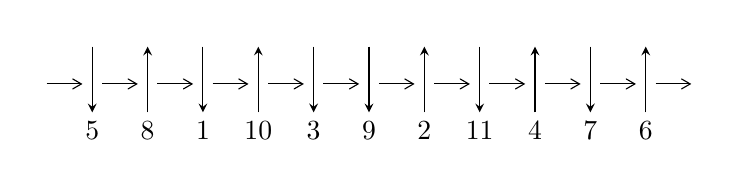
\begin{tikzpicture}[x=20pt, y=17pt]
	% nodes
	\node (C0) at (0, 0) {};
	\node (C1) at (1, 0) {};
	\node (C1U) at (1, +1) {};
	\node (C1D) at (1, -1) {5};

	\node (C2) at (2, 0) {};
	\node (C2U) at (2, +1) {};
	\node (C2D) at (2, -1) {8};

	\node (C3) at (3, 0) {};
	\node (C3U) at (3, +1) {};
	\node (C3D) at (3, -1) {1};

	\node (C4) at (4, 0) {};
	\node (C4U) at (4, +1) {};
	\node (C4D) at (4, -1) {10};

	\node (C5) at (5, 0) {};
	\node (C5U) at (5, +1) {};
	\node (C5D) at (5, -1) {3};

	\node (C6) at (6, 0) {};
	\node (C6U) at (6, +1) {};
	\node (C6D) at (6, -1) {9};

	\node (C7) at (7, 0) {};
	\node (C7U) at (7, +1) {};
	\node (C7D) at (7, -1) {2};

	\node (C8) at (8, 0) {};
	\node (C8U) at (8, +1) {};
	\node (C8D) at (8, -1) {11};

	\node (C9) at (9, 0) {};
	\node (C9U) at (9, +1) {};
	\node (C9D) at (9, -1) {4};

	\node (C10) at (10, 0) {};
	\node (C10U) at (10, +1) {};
	\node (C10D) at (10, -1) {7};

	\node (C11) at (11, 0) {};
	\node (C11U) at (11, +1) {};
	\node (C11D) at (11, -1) {6};
	\node (C12) at (12, 0) {};

	% arrows
	\draw[->,>={angle 60}]
	(C0) edge (C1) (C1) edge (C2) (C2) edge (C3) (C3) edge (C4) (C4) edge (C5) (C5) edge (C6) (C6) edge (C7) (C7) edge (C8) (C8) edge (C9) (C9) edge (C10) (C10) edge (C11) (C11) edge (C12) ;	\draw[->,>=stealth]
	(C1U) edge (C1D) (C2D) edge (C2U) (C3U) edge (C3D) (C4D) edge (C4U) (C5U) edge (C5D) (C6U) edge (C6D) (C7D) edge (C7U) (C8U) edge (C8D) (C9D) edge (C9U) (C10U) edge (C10D) (C11D) edge (C11U) ;
	\end{tikzpicture} \\
\hhline{~~} \\& 
\textbf{Solving Sequence} \\ \cline{2-2} 
 &
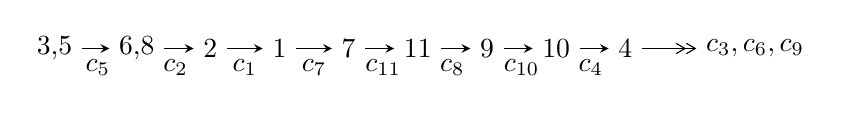
\begin{tikzpicture}[x=25pt, y=7pt]
	% node
	\node (A0) at (-1/8, 0) {3,5};
	\node (A1) at (17/16, 0) {6,8};
	\node (A2) at (17/8, 0) {2};
	\node (A3) at (25/8, 0) {1};
	\node (A4) at (33/8, 0) {7};
	\node (A5) at (41/8, 0) {11};
	\node (A6) at (49/8, 0) {9};
	\node (A7) at (57/8, 0) {10};
	\node (A8) at (65/8, 0) {4};
	\node (C1) at (1/2, -1) {$c_{5}$};
	\node (C2) at (13/8, -1) {$c_{2}$};
	\node (C3) at (21/8, -1) {$c_{1}$};
	\node (C4) at (29/8, -1) {$c_{7}$};
	\node (C5) at (37/8, -1) {$c_{11}$};
	\node (C6) at (45/8, -1) {$c_{8}$};
	\node (C7) at (53/8, -1) {$c_{10}$};
	\node (C8) at (61/8, -1) {$c_{4}$};
	\node (A9) at (10, 0) {$c_{3},c_{6},c_{9}$};

	% edge
	\draw[->,>=stealth]	
	(A0) edge (A1) (A1) edge (A2) (A2) edge (A3) (A3) edge (A4) (A4) edge (A5) (A5) edge (A6) (A6) edge (A7) (A7) edge (A8) ;
	\draw[->>,>={angle 60}]	
	(A8) edge (A9);
\end{tikzpicture} \\ 

\end{tabular} \\

\footnotetext{
The image of knot diagram is generated by the software ``\textbf{Draw programme}" developed by Andrew Bartholomew(\url{http://www.layer8.co.uk/maths/draw/index.htm\#Running-draw}), where we modified some parts for our purpose(\url{https://github.com/CATsTAILs/LinksPainter}).
}\phantom \\ \newline 
\centering \textbf{Ideals for irreducible components\footnotemark of $X_{\text{par}}$} 
 
\begin{align*}
I^u_{1}&=\langle 
-11 u^{14}-4 u^{13}+\cdots+18 b+5,\;10 u^{14}+9 u^{12}+\cdots+18 a-18,\\
\phantom{I^u_{1}}&\phantom{= \langle  }u^{15}+2 u^{13}+2 u^{12}+8 u^{11}+4 u^{10}+16 u^9+13 u^8+21 u^7+12 u^6+18 u^5+6 u^4+6 u^3-1\rangle \\
I^u_{2}&=\langle 
-1.37804\times10^{45} u^{35}-1.80053\times10^{44} u^{34}+\cdots+3.99041\times10^{45} b-1.10674\times10^{46},\\
\phantom{I^u_{2}}&\phantom{= \langle  }3.65397\times10^{45} u^{35}-4.93039\times10^{45} u^{34}+\cdots+3.99041\times10^{45} a+1.27280\times10^{45},\;u^{36}- u^{35}+\cdots-2 u+1\rangle \\
I^u_{3}&=\langle 
1.73314\times10^{71} u^{35}-1.61154\times10^{72} u^{34}+\cdots+1.23451\times10^{71} b+2.96287\times10^{71},\\
\phantom{I^u_{3}}&\phantom{= \langle  }-2.28749\times10^{71} u^{35}+1.95052\times10^{72} u^{34}+\cdots+1.23451\times10^{71} a-2.50099\times10^{72},\\
\phantom{I^u_{3}}&\phantom{= \langle  }u^{36}-10 u^{35}+\cdots-6 u-1\rangle \\
I^u_{4}&=\langle 
-61 u^9+5 u^8-23 u^7-223 u^6-204 u^5+3 u^4-340 u^3-294 u^2+53 b+46 u-34,\\
\phantom{I^u_{4}}&\phantom{= \langle  }24 u^9-15 u^8+16 u^7+86 u^6+29 u^5-9 u^4+172 u^3+34 u^2+53 a-32 u+102,\\
\phantom{I^u_{4}}&\phantom{= \langle  }u^{10}+4 u^7+4 u^6- u^5+5 u^4+7 u^3- u^2- u+1\rangle \\
I^u_{5}&=\langle 
u^5- u^3+u^2+b+u-1,\;- u^5+u^4+u^3-2 u^2+a+2,\;u^6- u^5+2 u^3- u+1\rangle \\
I^u_{6}&=\langle 
- u^5+2 u^4+u^2+2 b-3 u+1,\;- u^5+3 u^4-2 u^3+2 u^2+2 a-8 u+7,\;u^6-2 u^5-2 u^3+5 u^2-2 u-1\rangle \\
I^u_{7}&=\langle 
-17597088363 u^{11}+49269694805 u^{10}+\cdots+102937123333 b-11160459778,\\
\phantom{I^u_{7}}&\phantom{= \langle  }231997276705 u^{11}-468551566961 u^{10}+\cdots+102937123333 a-3200274870268,\\
\phantom{I^u_{7}}&\phantom{= \langle  }u^{12}-2 u^{11}-22 u^{10}-36 u^9-6 u^8+58 u^7+35 u^6-80 u^5-142 u^4-120 u^3-58 u^2-12 u+1\rangle \\
I^u_{8}&=\langle 
-3839279 u^{11}+8525704 u^{10}+\cdots+9619063 b-14981729,\\
\phantom{I^u_{8}}&\phantom{= \langle  }21714338 u^{11}-64033521 u^{10}+\cdots+28857189 a+1783311,\\
\phantom{I^u_{8}}&\phantom{= \langle  }u^{12}-3 u^{11}-4 u^{10}+8 u^9+10 u^8-12 u^7-33 u^6+50 u^5+2 u^4-44 u^3+25 u^2-3\rangle \\
I^u_{9}&=\langle 
b-1,\;a,\;u+1\rangle \\
I^u_{10}&=\langle 
b-1,\;a+u-3,\;u^2-2 u-1\rangle \\
\end{align*}\\
\begin{align*}
I^u_{11}&=\langle 
b,\;a-1,\;u-1\rangle \\
I^u_{12}&=\langle 
b-1,\;a-1,\;u-1\rangle \\
I^u_{13}&=\langle 
b+1,\;a-1,\;u+1\rangle \\
\\
I^v_{1}&=\langle 
a,\;b+1,\;v-1\rangle \\
\end{align*}
\raggedright * 14 irreducible components of $\dim_{\mathbb{C}}=0$, with total 140 representations.\\
\footnotetext{All coefficients of polynomials are rational numbers. But the coefficients are sometimes approximated in decimal forms when there is not enough margin.}
\newpage
\renewcommand{\arraystretch}{1}
\centering \section*{I. $I^u_{1}= \langle -11 u^{14}-4 u^{13}+\cdots+18 b+5,\;10 u^{14}+9 u^{12}+\cdots+18 a-18,\;u^{15}+2 u^{13}+\cdots+6 u^3-1 \rangle$}
\flushleft \textbf{(i) Arc colorings}\\
\begin{tabular}{m{7pt} m{180pt} m{7pt} m{180pt} }
\flushright $a_{3}=$&$\begin{pmatrix}0\\u\end{pmatrix}$ \\
\flushright $a_{5}=$&$\begin{pmatrix}1\\0\end{pmatrix}$ \\
\flushright $a_{6}=$&$\begin{pmatrix}1\\u^2\end{pmatrix}$ \\
\flushright $a_{8}=$&$\begin{pmatrix}-\frac{5}{9} u^{14}-\frac{1}{2} u^{12}+\cdots+\frac{23}{18} u+1\\\frac{11}{18} u^{14}+\frac{2}{9} u^{13}+\cdots-\frac{11}{9} u-\frac{5}{18}\end{pmatrix}$ \\
\flushright $a_{2}=$&$\begin{pmatrix}-\frac{5}{18} u^{14}-\frac{1}{3} u^{12}+\cdots-\frac{7}{9} u-\frac{2}{3}\\\frac{5}{18} u^{14}+\frac{1}{3} u^{12}+\cdots+\frac{7}{9} u-\frac{1}{3}\end{pmatrix}$ \\
\flushright $a_{1}=$&$\begin{pmatrix}-1\\\frac{5}{18} u^{14}+\frac{1}{3} u^{12}+\cdots+\frac{7}{9} u-\frac{1}{3}\end{pmatrix}$ \\
\flushright $a_{7}=$&$\begin{pmatrix}-0.222222 u^{14}-0.277778 u^{13}+\cdots-0.722222 u+1.55556\\\frac{5}{18} u^{14}-\frac{1}{9} u^{13}+\cdots-\frac{2}{9} u-\frac{5}{18}\end{pmatrix}$ \\
\flushright $a_{11}=$&$\begin{pmatrix}-\frac{5}{18} u^{14}-\frac{1}{3} u^{12}+\cdots-\frac{7}{9} u-\frac{2}{3}\\\frac{1}{2} u^{14}-\frac{1}{3} u^{13}+\cdots+\frac{1}{2} u-\frac{1}{3}\end{pmatrix}$ \\
\flushright $a_{9}=$&$\begin{pmatrix}-0.555556 u^{14}+0.222222 u^{13}+\cdots+0.611111 u+0.722222\\\frac{5}{18} u^{14}-\frac{5}{18} u^{13}+\cdots-\frac{14}{9} u+\frac{2}{9}\end{pmatrix}$ \\
\flushright $a_{10}=$&$\begin{pmatrix}-0.0555556 u^{14}-0.222222 u^{13}+\cdots-0.0555556 u-0.722222\\\frac{11}{18} u^{13}+u^{11}+\cdots+u-\frac{5}{9}\end{pmatrix}$ \\
\flushright $a_{4}=$&$\begin{pmatrix}- u\\-\frac{2}{9} u^{13}+\frac{1}{3} u^{12}+\cdots+\frac{2}{3} u+\frac{5}{18}\end{pmatrix}$\\ \flushright $a_{4}=$&$\begin{pmatrix}- u\\-\frac{2}{9} u^{13}+\frac{1}{3} u^{12}+\cdots+\frac{2}{3} u+\frac{5}{18}\end{pmatrix}$\\&\end{tabular}
\flushleft \textbf{(ii) Obstruction class $= -1$}\\~\\
\flushleft \textbf{(iii) Cusp Shapes $= \frac{55}{9} u^{14}-\frac{8}{9} u^{13}+\frac{29}{3} u^{12}+\frac{89}{9} u^{11}+\frac{385}{9} u^{10}+\frac{116}{9} u^9+\frac{223}{3} u^8+\frac{484}{9} u^7+\frac{748}{9} u^6+\frac{241}{9} u^5+\frac{511}{9} u^4+\frac{25}{9} u^3+\frac{112}{9} u^2-\frac{47}{9} u+\frac{25}{9}$}\\~\\
\newpage\renewcommand{\arraystretch}{1}
\flushleft \textbf{(iv) u-Polynomials at the component}\newline \\
\begin{tabular}{m{50pt}|m{274pt}}
Crossings & \hspace{64pt}u-Polynomials at each crossing \\
\hline $$\begin{aligned}c_{1},c_{10}\end{aligned}$$&$\begin{aligned}
&u^{15}+9 u^{14}+\cdots-32 u-16
\end{aligned}$\\
\hline $$\begin{aligned}c_{2},c_{4},c_{7}\\c_{9}\end{aligned}$$&$\begin{aligned}
&u^{15}-4 u^{13}+9 u^{11}-2 u^{10}-8 u^9+7 u^8+2 u^7-12 u^6+4 u^5+9 u^4-2 u-2
\end{aligned}$\\
\hline $$\begin{aligned}c_{3},c_{5},c_{6}\\c_{8}\end{aligned}$$&$\begin{aligned}
&u^{15}+2 u^{13}+\cdots+6 u^3-1
\end{aligned}$\\
\hline $$\begin{aligned}c_{11}\end{aligned}$$&$\begin{aligned}
&u^{15}+13 u^{14}+\cdots-416 u-64
\end{aligned}$\\
\hline
\end{tabular}\\~\\
\newpage\renewcommand{\arraystretch}{1}
\flushleft \textbf{(v) Riley Polynomials at the component}\newline \\
\begin{tabular}{m{50pt}|m{274pt}}
Crossings & \hspace{64pt}Riley Polynomials at each crossing \\
\hline $$\begin{aligned}c_{1},c_{10}\end{aligned}$$&$\begin{aligned}
&y^{15}-5 y^{14}+\cdots+384 y-256
\end{aligned}$\\
\hline $$\begin{aligned}c_{2},c_{4},c_{7}\\c_{9}\end{aligned}$$&$\begin{aligned}
&y^{15}-8 y^{14}+\cdots+4 y-4
\end{aligned}$\\
\hline $$\begin{aligned}c_{3},c_{5},c_{6}\\c_{8}\end{aligned}$$&$\begin{aligned}
&y^{15}+4 y^{14}+\cdots+12 y^2-1
\end{aligned}$\\
\hline $$\begin{aligned}c_{11}\end{aligned}$$&$\begin{aligned}
&y^{15}-7 y^{14}+\cdots+11264 y-4096
\end{aligned}$\\
\hline
\end{tabular}\\~\\
\newpage\flushleft \textbf{(vi) Complex Volumes and Cusp Shapes}
$$\begin{array}{c|c|c}  
\text{Solutions to }I^u_{1}& \I (\text{vol} + \sqrt{-1}CS) & \text{Cusp shape}\\
 \hline 
\begin{aligned}
u &= \phantom{-}0.375965 + 0.932481 I \\
a &= -0.022789 - 1.214510 I \\
b &= \phantom{-}0.76086 + 2.35797 I\end{aligned}
 & \phantom{-}5.04027 - 9.43708 I & \phantom{-}7.9635 + 11.7594 I \\ \hline\begin{aligned}
u &= \phantom{-}0.375965 - 0.932481 I \\
a &= -0.022789 + 1.214510 I \\
b &= \phantom{-}0.76086 - 2.35797 I\end{aligned}
 & \phantom{-}5.04027 + 9.43708 I & \phantom{-}7.9635 - 11.7594 I \\ \hline\begin{aligned}
u &= -0.770687 + 0.717882 I \\
a &= \phantom{-}0.585197 + 0.439087 I \\
b &= -0.78233 - 1.39703 I\end{aligned}
 & \phantom{-}0.48581 + 3.45966 I & \phantom{-}2.92722 - 6.50047 I \\ \hline\begin{aligned}
u &= -0.770687 - 0.717882 I \\
a &= \phantom{-}0.585197 - 0.439087 I \\
b &= -0.78233 + 1.39703 I\end{aligned}
 & \phantom{-}0.48581 - 3.45966 I & \phantom{-}2.92722 + 6.50047 I \\ \hline\begin{aligned}
u &= -0.017197 + 0.777026 I \\
a &= -0.70943 + 1.35975 I \\
b &= -0.32717 - 1.53341 I\end{aligned}
 & \phantom{-}4.09690 + 5.67488 I & \phantom{-}5.06867 - 6.10846 I \\ \hline\begin{aligned}
u &= -0.017197 - 0.777026 I \\
a &= -0.70943 - 1.35975 I \\
b &= -0.32717 + 1.53341 I\end{aligned}
 & \phantom{-}4.09690 - 5.67488 I & \phantom{-}5.06867 + 6.10846 I \\ \hline\begin{aligned}
u &= \phantom{-}0.483358 + 1.164780 I \\
a &= \phantom{-}0.793953 - 0.756191 I \\
b &= \phantom{-}0.527888 + 1.092680 I\end{aligned}
 & \phantom{-}5.64308 + 1.61043 I & \phantom{-}6.76634 + 1.00019 I \\ \hline\begin{aligned}
u &= \phantom{-}0.483358 - 1.164780 I \\
a &= \phantom{-}0.793953 + 0.756191 I \\
b &= \phantom{-}0.527888 - 1.092680 I\end{aligned}
 & \phantom{-}5.64308 - 1.61043 I & \phantom{-}6.76634 - 1.00019 I \\ \hline\begin{aligned}
u &= -0.442558 + 0.472159 I \\
a &= \phantom{-}0.761967 - 0.578478 I \\
b &= -0.096613 - 0.396023 I\end{aligned}
 & -0.61502 + 1.62852 I & -1.81112 - 4.54842 I \\ \hline\begin{aligned}
u &= -0.442558 - 0.472159 I \\
a &= \phantom{-}0.761967 + 0.578478 I \\
b &= -0.096613 + 0.396023 I\end{aligned}
 & -0.61502 - 1.62852 I & -1.81112 + 4.54842 I\\
 \hline 
 \end{array}$$\newpage$$\begin{array}{c|c|c}  
\text{Solutions to }I^u_{1}& \I (\text{vol} + \sqrt{-1}CS) & \text{Cusp shape}\\
 \hline 
\begin{aligned}
u &= -1.031270 + 0.943313 I \\
a &= -0.670358 + 0.362743 I \\
b &= -0.175859 - 0.100257 I\end{aligned}
 & -3.28483 + 7.08124 I & -3.75198 - 5.71793 I \\ \hline\begin{aligned}
u &= -1.031270 - 0.943313 I \\
a &= -0.670358 - 0.362743 I \\
b &= -0.175859 + 0.100257 I\end{aligned}
 & -3.28483 - 7.08124 I & -3.75198 + 5.71793 I \\ \hline\begin{aligned}
u &= \phantom{-}0.419879\phantom{ +0.000000I} \\
a &= \phantom{-}2.09302\phantom{ +0.000000I} \\
b &= -0.477344\phantom{ +0.000000I}\end{aligned}
 & \phantom{-}1.70444\phantom{ +0.000000I} & \phantom{-}5.76330\phantom{ +0.000000I} \\ \hline\begin{aligned}
u &= \phantom{-}1.19245 + 1.13162 I \\
a &= -0.285046 + 0.850536 I \\
b &= -0.66810 - 2.22561 I\end{aligned}
 & \phantom{-}2.5860 - 19.7120 I & \phantom{-}0.95572 + 10.39733 I \\ \hline\begin{aligned}
u &= \phantom{-}1.19245 - 1.13162 I \\
a &= -0.285046 - 0.850536 I \\
b &= -0.66810 + 2.22561 I\end{aligned}
 & \phantom{-}2.5860 + 19.7120 I & \phantom{-}0.95572 - 10.39733 I\\
 \hline 
 \end{array}$$\newpage\newpage\renewcommand{\arraystretch}{1}
\centering \section*{II. $I^u_{2}= \langle -1.38\times10^{45} u^{35}-1.80\times10^{44} u^{34}+\cdots+3.99\times10^{45} b-1.11\times10^{46},\;3.65\times10^{45} u^{35}-4.93\times10^{45} u^{34}+\cdots+3.99\times10^{45} a+1.27\times10^{45},\;u^{36}- u^{35}+\cdots-2 u+1 \rangle$}
\flushleft \textbf{(i) Arc colorings}\\
\begin{tabular}{m{7pt} m{180pt} m{7pt} m{180pt} }
\flushright $a_{3}=$&$\begin{pmatrix}0\\u\end{pmatrix}$ \\
\flushright $a_{5}=$&$\begin{pmatrix}1\\0\end{pmatrix}$ \\
\flushright $a_{6}=$&$\begin{pmatrix}1\\u^2\end{pmatrix}$ \\
\flushright $a_{8}=$&$\begin{pmatrix}-0.915688 u^{35}+1.23556 u^{34}+\cdots-5.91984 u-0.318965\\0.345337 u^{35}+0.0451214 u^{34}+\cdots-6.72198 u+2.77349\end{pmatrix}$ \\
\flushright $a_{2}=$&$\begin{pmatrix}-3.55283 u^{35}+4.15978 u^{34}+\cdots-10.7211 u-1.59357\\0.343747 u^{35}-0.453576 u^{34}+\cdots-3.02752 u+0.528741\end{pmatrix}$ \\
\flushright $a_{1}=$&$\begin{pmatrix}-3.20909 u^{35}+3.70621 u^{34}+\cdots-13.7486 u-1.06483\\0.343747 u^{35}-0.453576 u^{34}+\cdots-3.02752 u+0.528741\end{pmatrix}$ \\
\flushright $a_{7}=$&$\begin{pmatrix}0.262533 u^{35}+0.323253 u^{34}+\cdots-10.4090 u+6.48551\\-0.282683 u^{35}+0.688828 u^{34}+\cdots-7.63695 u+1.19971\end{pmatrix}$ \\
\flushright $a_{11}=$&$\begin{pmatrix}-3.09336 u^{35}+3.63567 u^{34}+\cdots-6.51773 u-2.09069\\0.468774 u^{35}-0.540153 u^{34}+\cdots-3.05287 u+0.483555\end{pmatrix}$ \\
\flushright $a_{9}=$&$\begin{pmatrix}-0.373382 u^{35}+1.27775 u^{34}+\cdots-14.1973 u+2.77440\\0.273958 u^{35}-0.0694172 u^{34}+\cdots-5.30088 u+2.30472\end{pmatrix}$ \\
\flushright $a_{10}=$&$\begin{pmatrix}-2.31277 u^{35}+2.47738 u^{34}+\cdots-18.4300 u-0.137385\\0.0179996 u^{35}-0.268681 u^{34}+\cdots+5.18656 u-1.68120\end{pmatrix}$ \\
\flushright $a_{4}=$&$\begin{pmatrix}1.78549 u^{35}-1.68467 u^{34}+\cdots-7.57950 u+4.97500\\1.01596 u^{35}-1.06117 u^{34}+\cdots+5.42208 u+0.378941\end{pmatrix}$\\ \flushright $a_{4}=$&$\begin{pmatrix}1.78549 u^{35}-1.68467 u^{34}+\cdots-7.57950 u+4.97500\\1.01596 u^{35}-1.06117 u^{34}+\cdots+5.42208 u+0.378941\end{pmatrix}$\\&\end{tabular}
\flushleft \textbf{(ii) Obstruction class $= -1$}\\~\\
\flushleft \textbf{(iii) Cusp Shapes $= -5.15842 u^{35}+3.75096 u^{34}+\cdots+33.9670 u-14.9765$}\\~\\
\newpage\renewcommand{\arraystretch}{1}
\flushleft \textbf{(iv) u-Polynomials at the component}\newline \\
\begin{tabular}{m{50pt}|m{274pt}}
Crossings & \hspace{64pt}u-Polynomials at each crossing \\
\hline $$\begin{aligned}c_{1},c_{10}\end{aligned}$$&$\begin{aligned}
&(u^{18}-4 u^{17}+\cdots+4 u^2+1)^{2}
\end{aligned}$\\
\hline $$\begin{aligned}c_{2},c_{4},c_{7}\\c_{9}\end{aligned}$$&$\begin{aligned}
&u^{36}+3 u^{35}+\cdots+34 u+13
\end{aligned}$\\
\hline $$\begin{aligned}c_{3},c_{5},c_{6}\\c_{8}\end{aligned}$$&$\begin{aligned}
&u^{36}- u^{35}+\cdots-2 u+1
\end{aligned}$\\
\hline $$\begin{aligned}c_{11}\end{aligned}$$&$\begin{aligned}
&(u^{18}-5 u^{17}+\cdots-8 u+1)^{2}
\end{aligned}$\\
\hline
\end{tabular}\\~\\
\newpage\renewcommand{\arraystretch}{1}
\flushleft \textbf{(v) Riley Polynomials at the component}\newline \\
\begin{tabular}{m{50pt}|m{274pt}}
Crossings & \hspace{64pt}Riley Polynomials at each crossing \\
\hline $$\begin{aligned}c_{1},c_{10}\end{aligned}$$&$\begin{aligned}
&(y^{18}+10 y^{17}+\cdots+8 y+1)^{2}
\end{aligned}$\\
\hline $$\begin{aligned}c_{2},c_{4},c_{7}\\c_{9}\end{aligned}$$&$\begin{aligned}
&y^{36}-15 y^{35}+\cdots+40 y+169
\end{aligned}$\\
\hline $$\begin{aligned}c_{3},c_{5},c_{6}\\c_{8}\end{aligned}$$&$\begin{aligned}
&y^{36}- y^{35}+\cdots+28 y+1
\end{aligned}$\\
\hline $$\begin{aligned}c_{11}\end{aligned}$$&$\begin{aligned}
&(y^{18}+3 y^{17}+\cdots-8 y+1)^{2}
\end{aligned}$\\
\hline
\end{tabular}\\~\\
\newpage\flushleft \textbf{(vi) Complex Volumes and Cusp Shapes}
$$\begin{array}{c|c|c}  
\text{Solutions to }I^u_{2}& \I (\text{vol} + \sqrt{-1}CS) & \text{Cusp shape}\\
 \hline 
\begin{aligned}
u &= -0.363120 + 1.008320 I \\
a &= \phantom{-}0.026422 + 1.101700 I \\
b &= \phantom{-}0.70580 - 1.91504 I\end{aligned}
 & \phantom{-}2.57204 + 5.31192 I & \phantom{-}3.36040 - 8.00060 I \\ \hline\begin{aligned}
u &= -0.363120 - 1.008320 I \\
a &= \phantom{-}0.026422 - 1.101700 I \\
b &= \phantom{-}0.70580 + 1.91504 I\end{aligned}
 & \phantom{-}2.57204 - 5.31192 I & \phantom{-}3.36040 + 8.00060 I \\ \hline\begin{aligned}
u &= \phantom{-}0.649836 + 0.632824 I \\
a &= \phantom{-}0.608719 + 0.180629 I \\
b &= -0.783167 + 0.542527 I\end{aligned}
 & \phantom{-}2.57204 - 5.31192 I & \phantom{-}3.36040 + 8.00060 I \\ \hline\begin{aligned}
u &= \phantom{-}0.649836 - 0.632824 I \\
a &= \phantom{-}0.608719 - 0.180629 I \\
b &= -0.783167 - 0.542527 I\end{aligned}
 & \phantom{-}2.57204 + 5.31192 I & \phantom{-}3.36040 - 8.00060 I \\ \hline\begin{aligned}
u &= \phantom{-}0.893795 + 0.123771 I \\
a &= -0.806277 - 0.142896 I \\
b &= -0.470358 - 1.315610 I\end{aligned}
 & \phantom{-}3.30139 + 5.60580 I & \phantom{-}4.21097 - 5.33069 I \\ \hline\begin{aligned}
u &= \phantom{-}0.893795 - 0.123771 I \\
a &= -0.806277 + 0.142896 I \\
b &= -0.470358 + 1.315610 I\end{aligned}
 & \phantom{-}3.30139 - 5.60580 I & \phantom{-}4.21097 + 5.33069 I \\ \hline\begin{aligned}
u &= -0.440875 + 1.024740 I \\
a &= \phantom{-}0.025375 + 1.272790 I \\
b &= \phantom{-}0.33726 - 1.60649 I\end{aligned}
 & \phantom{-}3.30139 + 5.60580 I & \phantom{-}4.21097 - 5.33069 I \\ \hline\begin{aligned}
u &= -0.440875 - 1.024740 I \\
a &= \phantom{-}0.025375 - 1.272790 I \\
b &= \phantom{-}0.33726 + 1.60649 I\end{aligned}
 & \phantom{-}3.30139 - 5.60580 I & \phantom{-}4.21097 + 5.33069 I \\ \hline\begin{aligned}
u &= \phantom{-}0.517386 + 0.999523 I \\
a &= \phantom{-}0.149927 - 1.060780 I \\
b &= \phantom{-}0.04630 + 2.23105 I\end{aligned}
 & \phantom{-}5.05604 - 1.80030 I & \phantom{-}7.45000 + 3.46748 I \\ \hline\begin{aligned}
u &= \phantom{-}0.517386 - 0.999523 I \\
a &= \phantom{-}0.149927 + 1.060780 I \\
b &= \phantom{-}0.04630 - 2.23105 I\end{aligned}
 & \phantom{-}5.05604 + 1.80030 I & \phantom{-}7.45000 - 3.46748 I\\
 \hline 
 \end{array}$$\newpage$$\begin{array}{c|c|c}  
\text{Solutions to }I^u_{2}& \I (\text{vol} + \sqrt{-1}CS) & \text{Cusp shape}\\
 \hline 
\begin{aligned}
u &= \phantom{-}0.850004 + 0.786233 I \\
a &= -0.268215 - 0.726745 I \\
b &= -0.028148 + 0.754872 I\end{aligned}
 & \phantom{-}2.75241 - 3.93541 I & \phantom{-}2.90741 + 5.36629 I \\ \hline\begin{aligned}
u &= \phantom{-}0.850004 - 0.786233 I \\
a &= -0.268215 + 0.726745 I \\
b &= -0.028148 - 0.754872 I\end{aligned}
 & \phantom{-}2.75241 + 3.93541 I & \phantom{-}2.90741 - 5.36629 I \\ \hline\begin{aligned}
u &= \phantom{-}0.298814 + 0.783563 I \\
a &= \phantom{-}0.584126 + 0.283863 I \\
b &= -0.179299 - 0.216656 I\end{aligned}
 & \phantom{-}1.88210 + 1.75570 I & \phantom{-}3.07518 - 1.06674 I \\ \hline\begin{aligned}
u &= \phantom{-}0.298814 - 0.783563 I \\
a &= \phantom{-}0.584126 - 0.283863 I \\
b &= -0.179299 + 0.216656 I\end{aligned}
 & \phantom{-}1.88210 - 1.75570 I & \phantom{-}3.07518 + 1.06674 I \\ \hline\begin{aligned}
u &= -0.095278 + 0.825512 I \\
a &= \phantom{-}1.87436 + 0.04602 I \\
b &= -0.009002 - 0.144399 I\end{aligned}
 & -1.19542 - 1.15621 I & \phantom{-}10.86918 - 2.44420 I \\ \hline\begin{aligned}
u &= -0.095278 - 0.825512 I \\
a &= \phantom{-}1.87436 - 0.04602 I \\
b &= -0.009002 + 0.144399 I\end{aligned}
 & -1.19542 + 1.15621 I & \phantom{-}10.86918 + 2.44420 I \\ \hline\begin{aligned}
u &= \phantom{-}0.437518 + 1.136460 I \\
a &= \phantom{-}0.512918 - 1.258620 I \\
b &= \phantom{-}0.45023 + 1.44725 I\end{aligned}
 & \phantom{-}7.02166 - 7.49599 I & \phantom{-}6.57969 + 7.14836 I \\ \hline\begin{aligned}
u &= \phantom{-}0.437518 - 1.136460 I \\
a &= \phantom{-}0.512918 + 1.258620 I \\
b &= \phantom{-}0.45023 - 1.44725 I\end{aligned}
 & \phantom{-}7.02166 + 7.49599 I & \phantom{-}6.57969 - 7.14836 I \\ \hline\begin{aligned}
u &= -0.371712 + 1.181350 I \\
a &= \phantom{-}0.390182 + 0.870496 I \\
b &= \phantom{-}0.67521 - 1.35698 I\end{aligned}
 & \phantom{-}2.75241 + 3.93541 I & \phantom{-}2.90741 - 5.36629 I \\ \hline\begin{aligned}
u &= -0.371712 - 1.181350 I \\
a &= \phantom{-}0.390182 - 0.870496 I \\
b &= \phantom{-}0.67521 + 1.35698 I\end{aligned}
 & \phantom{-}2.75241 - 3.93541 I & \phantom{-}2.90741 + 5.36629 I\\
 \hline 
 \end{array}$$\newpage$$\begin{array}{c|c|c}  
\text{Solutions to }I^u_{2}& \I (\text{vol} + \sqrt{-1}CS) & \text{Cusp shape}\\
 \hline 
\begin{aligned}
u &= \phantom{-}0.972609 + 0.975530 I \\
a &= -0.804652 - 0.466962 I \\
b &= \phantom{-}0.0875024 + 0.0540753 I\end{aligned}
 & -0.55505 - 12.95420 I & -1.0000 + 8.63684 I \\ \hline\begin{aligned}
u &= \phantom{-}0.972609 - 0.975530 I \\
a &= -0.804652 + 0.466962 I \\
b &= \phantom{-}0.0875024 - 0.0540753 I\end{aligned}
 & -0.55505 + 12.95420 I & -1.0000 - 8.63684 I \\ \hline\begin{aligned}
u &= -1.375460 + 0.143710 I \\
a &= \phantom{-}0.532601 + 0.386317 I \\
b &= \phantom{-}0.755723 - 0.967094 I\end{aligned}
 & -2.74089 + 1.92073 I & -7.73857 - 5.49648 I \\ \hline\begin{aligned}
u &= -1.375460 - 0.143710 I \\
a &= \phantom{-}0.532601 - 0.386317 I \\
b &= \phantom{-}0.755723 + 0.967094 I\end{aligned}
 & -2.74089 - 1.92073 I & -7.73857 + 5.49648 I \\ \hline\begin{aligned}
u &= \phantom{-}0.338423 + 0.447370 I \\
a &= \phantom{-}0.36194 - 1.95892 I \\
b &= -0.396182 + 1.120630 I\end{aligned}
 & \phantom{-}1.88210 - 1.75570 I & \phantom{-}3.07518 + 1.06674 I \\ \hline\begin{aligned}
u &= \phantom{-}0.338423 - 0.447370 I \\
a &= \phantom{-}0.36194 + 1.95892 I \\
b &= -0.396182 - 1.120630 I\end{aligned}
 & \phantom{-}1.88210 + 1.75570 I & \phantom{-}3.07518 - 1.06674 I \\ \hline\begin{aligned}
u &= -0.092953 + 0.387873 I \\
a &= \phantom{-}2.70253 - 0.69095 I \\
b &= \phantom{-}0.598829 - 0.213056 I\end{aligned}
 & -2.74089 + 1.92073 I & -7.73857 - 5.49648 I \\ \hline\begin{aligned}
u &= -0.092953 - 0.387873 I \\
a &= \phantom{-}2.70253 + 0.69095 I \\
b &= \phantom{-}0.598829 + 0.213056 I\end{aligned}
 & -2.74089 - 1.92073 I & -7.73857 + 5.49648 I \\ \hline\begin{aligned}
u &= -0.164240 + 0.304020 I \\
a &= \phantom{-}0.30937 + 3.57193 I \\
b &= -0.77904 - 1.26752 I\end{aligned}
 & \phantom{-}5.05604 - 1.80030 I & \phantom{-}7.45000 + 3.46748 I \\ \hline\begin{aligned}
u &= -0.164240 - 0.304020 I \\
a &= \phantom{-}0.30937 - 3.57193 I \\
b &= -0.77904 + 1.26752 I\end{aligned}
 & \phantom{-}5.05604 + 1.80030 I & \phantom{-}7.45000 - 3.46748 I\\
 \hline 
 \end{array}$$\newpage$$\begin{array}{c|c|c}  
\text{Solutions to }I^u_{2}& \I (\text{vol} + \sqrt{-1}CS) & \text{Cusp shape}\\
 \hline 
\begin{aligned}
u &= \phantom{-}1.40474 + 0.96008 I \\
a &= -0.456383 + 0.579963 I \\
b &= -0.73214 - 2.09422 I\end{aligned}
 & \phantom{-}7.02166 - 7.49599 I & \phantom{-0.000000 } 0 \\ \hline\begin{aligned}
u &= \phantom{-}1.40474 - 0.96008 I \\
a &= -0.456383 - 0.579963 I \\
b &= -0.73214 + 2.09422 I\end{aligned}
 & \phantom{-}7.02166 + 7.49599 I & \phantom{-0.000000 } 0 \\ \hline\begin{aligned}
u &= -1.26242 + 1.17225 I \\
a &= -0.270237 - 0.743976 I \\
b &= -0.67214 + 2.21899 I\end{aligned}
 & -0.55505 + 12.95420 I & \phantom{-0.000000 } 0 \\ \hline\begin{aligned}
u &= -1.26242 - 1.17225 I \\
a &= -0.270237 + 0.743976 I \\
b &= -0.67214 - 2.21899 I\end{aligned}
 & -0.55505 - 12.95420 I & \phantom{-0.000000 } 0 \\ \hline\begin{aligned}
u &= -1.69707 + 0.32713 I \\
a &= -0.472709 - 0.238795 I \\
b &= -1.10737 + 1.60482 I\end{aligned}
 & -1.19542 + 1.15621 I & \phantom{-0.000000 } 0 \\ \hline\begin{aligned}
u &= -1.69707 - 0.32713 I \\
a &= -0.472709 + 0.238795 I \\
b &= -1.10737 - 1.60482 I\end{aligned}
 & -1.19542 - 1.15621 I & \phantom{-0.000000 } 0\\
 \hline 
 \end{array}$$\newpage\newpage\renewcommand{\arraystretch}{1}
\centering \section*{III. $I^u_{3}= \langle 1.73\times10^{71} u^{35}-1.61\times10^{72} u^{34}+\cdots+1.23\times10^{71} b+2.96\times10^{71},\;-2.29\times10^{71} u^{35}+1.95\times10^{72} u^{34}+\cdots+1.23\times10^{71} a-2.50\times10^{72},\;u^{36}-10 u^{35}+\cdots-6 u-1 \rangle$}
\flushleft \textbf{(i) Arc colorings}\\
\begin{tabular}{m{7pt} m{180pt} m{7pt} m{180pt} }
\flushright $a_{3}=$&$\begin{pmatrix}0\\u\end{pmatrix}$ \\
\flushright $a_{5}=$&$\begin{pmatrix}1\\0\end{pmatrix}$ \\
\flushright $a_{6}=$&$\begin{pmatrix}1\\u^2\end{pmatrix}$ \\
\flushright $a_{8}=$&$\begin{pmatrix}1.85295 u^{35}-15.7999 u^{34}+\cdots+13.9344 u+20.2589\\-1.40390 u^{35}+13.0541 u^{34}+\cdots-19.0944 u-2.40003\end{pmatrix}$ \\
\flushright $a_{2}=$&$\begin{pmatrix}-1.02308 u^{35}+12.5666 u^{34}+\cdots-17.7060 u+40.2995\\-1.98793 u^{35}+18.5611 u^{34}+\cdots-21.0095 u-2.60561\end{pmatrix}$ \\
\flushright $a_{1}=$&$\begin{pmatrix}-3.01101 u^{35}+31.1278 u^{34}+\cdots-38.7154 u+37.6939\\-1.98793 u^{35}+18.5611 u^{34}+\cdots-21.0095 u-2.60561\end{pmatrix}$ \\
\flushright $a_{7}=$&$\begin{pmatrix}12.7714 u^{35}-126.136 u^{34}+\cdots+173.374 u-58.1830\\0.117701 u^{35}-1.17964 u^{34}+\cdots+0.298887 u-0.237165\end{pmatrix}$ \\
\flushright $a_{11}=$&$\begin{pmatrix}-1.01828 u^{35}+12.4254 u^{34}+\cdots-14.6110 u+41.3172\\-1.24273 u^{35}+11.5677 u^{34}+\cdots-11.6668 u-1.38062\end{pmatrix}$ \\
\flushright $a_{9}=$&$\begin{pmatrix}9.38240 u^{35}-94.2192 u^{34}+\cdots+135.032 u-61.6432\\0.456694 u^{35}-4.47246 u^{34}+\cdots+6.95760 u+0.699328\end{pmatrix}$ \\
\flushright $a_{10}=$&$\begin{pmatrix}-26.5737 u^{35}+270.228 u^{34}+\cdots-395.140 u+223.633\\-0.323427 u^{35}+3.24528 u^{34}+\cdots-7.68584 u-0.142044\end{pmatrix}$ \\
\flushright $a_{4}=$&$\begin{pmatrix}-23.0908 u^{35}+234.477 u^{34}+\cdots-344.610 u+187.947\\0.952036 u^{35}-8.90987 u^{34}+\cdots+13.6977 u+2.55897\end{pmatrix}$\\ \flushright $a_{4}=$&$\begin{pmatrix}-23.0908 u^{35}+234.477 u^{34}+\cdots-344.610 u+187.947\\0.952036 u^{35}-8.90987 u^{34}+\cdots+13.6977 u+2.55897\end{pmatrix}$\\&\end{tabular}
\flushleft \textbf{(ii) Obstruction class $= -1$}\\~\\
\flushleft \textbf{(iii) Cusp Shapes $= 31.0394 u^{35}-320.627 u^{34}+\cdots+444.568 u-347.305$}\\~\\
\newpage\renewcommand{\arraystretch}{1}
\flushleft \textbf{(iv) u-Polynomials at the component}\newline \\
\begin{tabular}{m{50pt}|m{274pt}}
Crossings & \hspace{64pt}u-Polynomials at each crossing \\
\hline $$\begin{aligned}c_{1},c_{10}\end{aligned}$$&$\begin{aligned}
&(u^{18}- u^{17}+\cdots+8 u-1)^{2}
\end{aligned}$\\
\hline $$\begin{aligned}c_{2},c_{4},c_{7}\\c_{9}\end{aligned}$$&$\begin{aligned}
&(u^{18}-8 u^{16}+\cdots+2 u-1)^{2}
\end{aligned}$\\
\hline $$\begin{aligned}c_{3},c_{5},c_{6}\\c_{8}\end{aligned}$$&$\begin{aligned}
&u^{36}-10 u^{35}+\cdots-6 u-1
\end{aligned}$\\
\hline $$\begin{aligned}c_{11}\end{aligned}$$&$\begin{aligned}
&(u^9- u^8+3 u^7+u^6+u^5- u^4+2 u^3+u+1)^4
\end{aligned}$\\
\hline
\end{tabular}\\~\\
\newpage\renewcommand{\arraystretch}{1}
\flushleft \textbf{(v) Riley Polynomials at the component}\newline \\
\begin{tabular}{m{50pt}|m{274pt}}
Crossings & \hspace{64pt}Riley Polynomials at each crossing \\
\hline $$\begin{aligned}c_{1},c_{10}\end{aligned}$$&$\begin{aligned}
&(y^{18}-7 y^{17}+\cdots-32 y+1)^{2}
\end{aligned}$\\
\hline $$\begin{aligned}c_{2},c_{4},c_{7}\\c_{9}\end{aligned}$$&$\begin{aligned}
&(y^{18}-16 y^{17}+\cdots-18 y+1)^{2}
\end{aligned}$\\
\hline $$\begin{aligned}c_{3},c_{5},c_{6}\\c_{8}\end{aligned}$$&$\begin{aligned}
&y^{36}-42 y^{35}+\cdots-66 y+1
\end{aligned}$\\
\hline $$\begin{aligned}c_{11}\end{aligned}$$&$\begin{aligned}
&(y^9+5 y^8+13 y^7+7 y^6+17 y^5+11 y^4+4 y^3+6 y^2+y-1)^4
\end{aligned}$\\
\hline
\end{tabular}\\~\\
\newpage\flushleft \textbf{(vi) Complex Volumes and Cusp Shapes}
$$\begin{array}{c|c|c}  
\text{Solutions to }I^u_{3}& \I (\text{vol} + \sqrt{-1}CS) & \text{Cusp shape}\\
 \hline 
\begin{aligned}
u &= -1.03358\phantom{ +0.000000I} \\
a &= -0.814532\phantom{ +0.000000I} \\
b &= \phantom{-}2.17328\phantom{ +0.000000I}\end{aligned}
 & -0.410667\phantom{ +0.000000I} & -404.090\phantom{ +0.000000I} \\ \hline\begin{aligned}
u &= -0.974908 + 0.644375 I \\
a &= \phantom{-}0.649195 - 0.319150 I \\
b &= \phantom{-}0.464754 - 0.305283 I\end{aligned}
 & -2.62213 + 1.09146 I & \phantom{-0.000000 } 0. - 5.89503 I \\ \hline\begin{aligned}
u &= -0.974908 - 0.644375 I \\
a &= \phantom{-}0.649195 + 0.319150 I \\
b &= \phantom{-}0.464754 + 0.305283 I\end{aligned}
 & -2.62213 - 1.09146 I & \phantom{-0.000000 -}0. + 5.89503 I \\ \hline\begin{aligned}
u &= -1.210830 + 0.190950 I \\
a &= \phantom{-}0.379075 + 0.256363 I \\
b &= \phantom{-}0.329763 - 0.186088 I\end{aligned}
 & -2.62213 + 1.09146 I & \phantom{-0.000000 } 0. - 5.89503 I \\ \hline\begin{aligned}
u &= -1.210830 - 0.190950 I \\
a &= \phantom{-}0.379075 - 0.256363 I \\
b &= \phantom{-}0.329763 + 0.186088 I\end{aligned}
 & -2.62213 - 1.09146 I & \phantom{-0.000000 -}0. + 5.89503 I \\ \hline\begin{aligned}
u &= \phantom{-}0.972906 + 0.767071 I \\
a &= -0.541205 + 0.879014 I \\
b &= -0.93294 - 2.13800 I\end{aligned}
 & \phantom{-}2.94139 - 10.34380 I & \phantom{-0.000000 -}0. + 12.71172 I \\ \hline\begin{aligned}
u &= \phantom{-}0.972906 - 0.767071 I \\
a &= -0.541205 - 0.879014 I \\
b &= -0.93294 + 2.13800 I\end{aligned}
 & \phantom{-}2.94139 + 10.34380 I & \phantom{-0.000000 } 0. - 12.71172 I \\ \hline\begin{aligned}
u &= \phantom{-}1.202800 + 0.351550 I \\
a &= \phantom{-}0.934184 + 0.310379 I \\
b &= -0.368803 - 0.573213 I\end{aligned}
 & \phantom{-}1.62967 - 1.42694 I & \phantom{-0.000000 } 0 \\ \hline\begin{aligned}
u &= \phantom{-}1.202800 - 0.351550 I \\
a &= \phantom{-}0.934184 - 0.310379 I \\
b &= -0.368803 + 0.573213 I\end{aligned}
 & \phantom{-}1.62967 + 1.42694 I & \phantom{-0.000000 } 0 \\ \hline\begin{aligned}
u &= \phantom{-}0.687915 + 0.243994 I \\
a &= -1.08739 + 1.22141 I \\
b &= \phantom{-}0.64121 - 1.29222 I\end{aligned}
 & -0.92113 - 6.20293 I & -12.02897 + 1.29054 I\\
 \hline 
 \end{array}$$\newpage$$\begin{array}{c|c|c}  
\text{Solutions to }I^u_{3}& \I (\text{vol} + \sqrt{-1}CS) & \text{Cusp shape}\\
 \hline 
\begin{aligned}
u &= \phantom{-}0.687915 - 0.243994 I \\
a &= -1.08739 - 1.22141 I \\
b &= \phantom{-}0.64121 + 1.29222 I\end{aligned}
 & -0.92113 + 6.20293 I & -12.02897 - 1.29054 I \\ \hline\begin{aligned}
u &= -0.556413 + 0.468109 I \\
a &= -0.71488 - 2.04959 I \\
b &= -0.429966 + 0.930334 I\end{aligned}
 & \phantom{-}2.94139 + 10.34380 I & \phantom{-}0.42699 - 12.71172 I \\ \hline\begin{aligned}
u &= -0.556413 - 0.468109 I \\
a &= -0.71488 + 2.04959 I \\
b &= -0.429966 - 0.930334 I\end{aligned}
 & \phantom{-}2.94139 - 10.34380 I & \phantom{-}0.42699 + 12.71172 I \\ \hline\begin{aligned}
u &= \phantom{-}0.653523 + 0.259178 I \\
a &= \phantom{-}0.97344 - 1.45983 I \\
b &= \phantom{-}0.555400 + 0.282300 I\end{aligned}
 & \phantom{-}1.62967 + 1.42694 I & -3.03389 + 0.96634 I \\ \hline\begin{aligned}
u &= \phantom{-}0.653523 - 0.259178 I \\
a &= \phantom{-}0.97344 + 1.45983 I \\
b &= \phantom{-}0.555400 - 0.282300 I\end{aligned}
 & \phantom{-}1.62967 - 1.42694 I & -3.03389 - 0.96634 I \\ \hline\begin{aligned}
u &= -0.457113 + 0.422721 I \\
a &= -0.99106 - 1.58772 I \\
b &= -0.98611 + 1.70538 I\end{aligned}
 & \phantom{-}1.62967 + 1.42694 I & -3.03389 + 0.96634 I \\ \hline\begin{aligned}
u &= -0.457113 - 0.422721 I \\
a &= -0.99106 + 1.58772 I \\
b &= -0.98611 - 1.70538 I\end{aligned}
 & \phantom{-}1.62967 - 1.42694 I & -3.03389 - 0.96634 I \\ \hline\begin{aligned}
u &= -0.528987 + 0.241881 I \\
a &= \phantom{-}0.964352 - 0.009017 I \\
b &= \phantom{-}1.10558 + 1.36508 I\end{aligned}
 & -2.62213 - 1.09146 I & -4.31933 + 5.89503 I \\ \hline\begin{aligned}
u &= -0.528987 - 0.241881 I \\
a &= \phantom{-}0.964352 + 0.009017 I \\
b &= \phantom{-}1.10558 - 1.36508 I\end{aligned}
 & -2.62213 + 1.09146 I & -4.31933 - 5.89503 I \\ \hline\begin{aligned}
u &= \phantom{-}1.27165 + 0.63193 I \\
a &= \phantom{-}0.294180 - 0.085640 I \\
b &= \phantom{-}0.399780 + 0.320910 I\end{aligned}
 & -0.92113 - 6.20293 I & \phantom{-0.000000 } 0\\
 \hline 
 \end{array}$$\newpage$$\begin{array}{c|c|c}  
\text{Solutions to }I^u_{3}& \I (\text{vol} + \sqrt{-1}CS) & \text{Cusp shape}\\
 \hline 
\begin{aligned}
u &= \phantom{-}1.27165 - 0.63193 I \\
a &= \phantom{-}0.294180 + 0.085640 I \\
b &= \phantom{-}0.399780 - 0.320910 I\end{aligned}
 & -0.92113 + 6.20293 I & \phantom{-0.000000 } 0 \\ \hline\begin{aligned}
u &= \phantom{-}0.553048 + 0.027251 I \\
a &= -0.83551 - 1.27783 I \\
b &= \phantom{-}0.541322 + 0.585100 I\end{aligned}
 & -2.62213 - 1.09146 I & -4.31933 + 5.89503 I \\ \hline\begin{aligned}
u &= \phantom{-}0.553048 - 0.027251 I \\
a &= -0.83551 + 1.27783 I \\
b &= \phantom{-}0.541322 - 0.585100 I\end{aligned}
 & -2.62213 + 1.09146 I & -4.31933 - 5.89503 I \\ \hline\begin{aligned}
u &= -0.96035 + 1.23478 I \\
a &= \phantom{-}0.120430 + 0.753486 I \\
b &= \phantom{-}0.84582 - 2.08861 I\end{aligned}
 & -0.92113 + 6.20293 I & \phantom{-0.000000 } 0 \\ \hline\begin{aligned}
u &= -0.96035 - 1.23478 I \\
a &= \phantom{-}0.120430 - 0.753486 I \\
b &= \phantom{-}0.84582 + 2.08861 I\end{aligned}
 & -0.92113 - 6.20293 I & \phantom{-0.000000 } 0 \\ \hline\begin{aligned}
u &= -0.020107 + 0.337379 I \\
a &= -0.302784 - 1.251190 I \\
b &= -0.97510 - 2.83519 I\end{aligned}
 & -0.92113 + 6.20293 I & -12.02897 - 1.29054 I \\ \hline\begin{aligned}
u &= -0.020107 - 0.337379 I \\
a &= -0.302784 + 1.251190 I \\
b &= -0.97510 + 2.83519 I\end{aligned}
 & -0.92113 - 6.20293 I & -12.02897 + 1.29054 I \\ \hline\begin{aligned}
u &= \phantom{-}1.24101 + 1.12995 I \\
a &= \phantom{-}0.274705 - 0.899412 I \\
b &= \phantom{-}0.45396 + 2.12603 I\end{aligned}
 & \phantom{-}2.94139 - 10.34380 I & \phantom{-0.000000 } 0 \\ \hline\begin{aligned}
u &= \phantom{-}1.24101 - 1.12995 I \\
a &= \phantom{-}0.274705 + 0.899412 I \\
b &= \phantom{-}0.45396 - 2.12603 I\end{aligned}
 & \phantom{-}2.94139 + 10.34380 I & \phantom{-0.000000 } 0 \\ \hline\begin{aligned}
u &= \phantom{-}0.70138 + 1.63277 I \\
a &= \phantom{-}0.091048 - 0.649406 I \\
b &= \phantom{-}0.21926 + 1.83471 I\end{aligned}
 & \phantom{-}1.62967 - 1.42694 I & \phantom{-0.000000 } 0\\
 \hline 
 \end{array}$$\newpage$$\begin{array}{c|c|c}  
\text{Solutions to }I^u_{3}& \I (\text{vol} + \sqrt{-1}CS) & \text{Cusp shape}\\
 \hline 
\begin{aligned}
u &= \phantom{-}0.70138 - 1.63277 I \\
a &= \phantom{-}0.091048 + 0.649406 I \\
b &= \phantom{-}0.21926 - 1.83471 I\end{aligned}
 & \phantom{-}1.62967 + 1.42694 I & \phantom{-0.000000 } 0 \\ \hline\begin{aligned}
u &= -0.127258\phantom{ +0.000000I} \\
a &= \phantom{-}18.2781\phantom{ +0.000000I} \\
b &= \phantom{-}0.120902\phantom{ +0.000000I}\end{aligned}
 & -0.410667\phantom{ +0.000000I} & -404.090\phantom{ +0.000000I} \\ \hline\begin{aligned}
u &= \phantom{-}1.41519 + 1.57427 I \\
a &= -0.533829 + 0.282886 I \\
b &= -1.01282 - 1.31300 I\end{aligned}
 & \phantom{-}2.94139 + 10.34380 I & \phantom{-0.000000 } 0 \\ \hline\begin{aligned}
u &= \phantom{-}1.41519 - 1.57427 I \\
a &= -0.533829 - 0.282886 I \\
b &= -1.01282 + 1.31300 I\end{aligned}
 & \phantom{-}2.94139 - 10.34380 I & \phantom{-0.000000 } 0 \\ \hline\begin{aligned}
u &= -2.25061\phantom{ +0.000000I} \\
a &= \phantom{-}1.03351\phantom{ +0.000000I} \\
b &= -0.263377\phantom{ +0.000000I}\end{aligned}
 & -0.410667\phantom{ +0.000000I} & \phantom{-0.000000 } 0 \\ \hline\begin{aligned}
u &= \phantom{-}5.43001\phantom{ +0.000000I} \\
a &= \phantom{-}0.155043\phantom{ +0.000000I} \\
b &= \phantom{-}6.26696\phantom{ +0.000000I}\end{aligned}
 & -0.410667\phantom{ +0.000000I} & \phantom{-0.000000 } 0\\
 \hline 
 \end{array}$$\newpage\newpage\renewcommand{\arraystretch}{1}
\centering \section*{IV. $I^u_{4}= \langle -61 u^9+5 u^8+\cdots+53 b-34,\;24 u^9-15 u^8+\cdots+53 a+102,\;u^{10}+4 u^7+4 u^6- u^5+5 u^4+7 u^3- u^2- u+1 \rangle$}
\flushleft \textbf{(i) Arc colorings}\\
\begin{tabular}{m{7pt} m{180pt} m{7pt} m{180pt} }
\flushright $a_{3}=$&$\begin{pmatrix}0\\u\end{pmatrix}$ \\
\flushright $a_{5}=$&$\begin{pmatrix}1\\0\end{pmatrix}$ \\
\flushright $a_{6}=$&$\begin{pmatrix}1\\u^2\end{pmatrix}$ \\
\flushright $a_{8}=$&$\begin{pmatrix}-0.452830 u^{9}+0.283019 u^{8}+\cdots+0.603774 u-1.92453\\1.15094 u^{9}-0.0943396 u^{8}+\cdots-0.867925 u+0.641509\end{pmatrix}$ \\
\flushright $a_{2}=$&$\begin{pmatrix}0.679245 u^{9}-0.924528 u^{8}+\cdots-3.90566 u+0.886792\\-0.679245 u^{9}+0.924528 u^{8}+\cdots+3.90566 u-1.88679\end{pmatrix}$ \\
\flushright $a_{1}=$&$\begin{pmatrix}-1\\-0.679245 u^{9}+0.924528 u^{8}+\cdots+3.90566 u-1.88679\end{pmatrix}$ \\
\flushright $a_{7}=$&$\begin{pmatrix}1.09434 u^{9}-0.433962 u^{8}+\cdots-1.79245 u-0.849057\\-0.679245 u^{9}+0.924528 u^{8}+\cdots+3.90566 u-0.886792\end{pmatrix}$ \\
\flushright $a_{11}=$&$\begin{pmatrix}0.679245 u^{9}-0.924528 u^{8}+\cdots-3.90566 u+0.886792\\-0.226415 u^{9}+0.641509 u^{8}+\cdots+2.30189 u-0.962264\end{pmatrix}$ \\
\flushright $a_{9}=$&$\begin{pmatrix}u^9+4 u^6+4 u^5- u^4+5 u^3+7 u^2- u-1\\0.433962 u^{9}-0.396226 u^{8}+\cdots-0.245283 u+1.09434\end{pmatrix}$ \\
\flushright $a_{10}=$&$\begin{pmatrix}-0.698113 u^{9}-0.188679 u^{8}+\cdots+0.264151 u+1.28302\\0.283019 u^{9}-0.301887 u^{8}+\cdots-2.37736 u+0.452830\end{pmatrix}$ \\
\flushright $a_{4}=$&$\begin{pmatrix}- u\\0.924528 u^{9}-0.452830 u^{8}+\cdots-1.56604 u+0.679245\end{pmatrix}$\\ \flushright $a_{4}=$&$\begin{pmatrix}- u\\0.924528 u^{9}-0.452830 u^{8}+\cdots-1.56604 u+0.679245\end{pmatrix}$\\&\end{tabular}
\flushleft \textbf{(ii) Obstruction class $= -1$}\\~\\
\flushleft \textbf{(iii) Cusp Shapes $= -\frac{199}{53} u^9+\frac{237}{53} u^8-\frac{274}{53} u^7-\frac{691}{53} u^6-\frac{13}{53} u^5+\frac{280}{53} u^4-\frac{1859}{53} u^3+\frac{14}{53} u^2+\frac{548}{53} u-\frac{647}{53}$}\\~\\
\newpage\renewcommand{\arraystretch}{1}
\flushleft \textbf{(iv) u-Polynomials at the component}\newline \\
\begin{tabular}{m{50pt}|m{274pt}}
Crossings & \hspace{64pt}u-Polynomials at each crossing \\
\hline $$\begin{aligned}c_{1},c_{10}\end{aligned}$$&$\begin{aligned}
&u^{10}+10 u^9+\cdots+131 u+29
\end{aligned}$\\
\hline $$\begin{aligned}c_{2},c_{4},c_{7}\\c_{9}\end{aligned}$$&$\begin{aligned}
&(u^5-2 u^3+u+1)^2
\end{aligned}$\\
\hline $$\begin{aligned}c_{3},c_{5},c_{6}\\c_{8}\end{aligned}$$&$\begin{aligned}
&u^{10}+4 u^7+4 u^6- u^5+5 u^4+7 u^3- u^2- u+1
\end{aligned}$\\
\hline $$\begin{aligned}c_{11}\end{aligned}$$&$\begin{aligned}
&(u^5+5 u^4+13 u^3+18 u^2+16 u+8)^2
\end{aligned}$\\
\hline
\end{tabular}\\~\\
\newpage\renewcommand{\arraystretch}{1}
\flushleft \textbf{(v) Riley Polynomials at the component}\newline \\
\begin{tabular}{m{50pt}|m{274pt}}
Crossings & \hspace{64pt}Riley Polynomials at each crossing \\
\hline $$\begin{aligned}c_{1},c_{10}\end{aligned}$$&$\begin{aligned}
&y^{10}-4 y^9+\cdots+877 y+841
\end{aligned}$\\
\hline $$\begin{aligned}c_{2},c_{4},c_{7}\\c_{9}\end{aligned}$$&$\begin{aligned}
&(y^5-4 y^4+6 y^3-4 y^2+y-1)^2
\end{aligned}$\\
\hline $$\begin{aligned}c_{3},c_{5},c_{6}\\c_{8}\end{aligned}$$&$\begin{aligned}
&y^{10}+8 y^8-6 y^7+22 y^6-15 y^5+39 y^4-53 y^3+25 y^2-3 y+1
\end{aligned}$\\
\hline $$\begin{aligned}c_{11}\end{aligned}$$&$\begin{aligned}
&(y^5+y^4+21 y^3+12 y^2-32 y-64)^2
\end{aligned}$\\
\hline
\end{tabular}\\~\\
\newpage\flushleft \textbf{(vi) Complex Volumes and Cusp Shapes}
$$\begin{array}{c|c|c}  
\text{Solutions to }I^u_{4}& \I (\text{vol} + \sqrt{-1}CS) & \text{Cusp shape}\\
 \hline 
\begin{aligned}
u &= -0.820200 + 0.152463 I \\
a &= -1.25990 - 0.71322 I \\
b &= \phantom{-}1.44173 + 0.78416 I\end{aligned}
 & \phantom{-}1.73183 + 9.10410 I & -2.74192 - 10.20249 I \\ \hline\begin{aligned}
u &= -0.820200 - 0.152463 I \\
a &= -1.25990 + 0.71322 I \\
b &= \phantom{-}1.44173 - 0.78416 I\end{aligned}
 & \phantom{-}1.73183 - 9.10410 I & -2.74192 + 10.20249 I \\ \hline\begin{aligned}
u &= \phantom{-}0.583652 + 1.118000 I \\
a &= -0.500000 + 0.957760 I \\
b &= -0.66223 - 1.77825 I\end{aligned}
 & \phantom{-}9.67856\phantom{ +0.000000I} & \phantom{-}7.93446 + 0. I\phantom{ +0.000000I} \\ \hline\begin{aligned}
u &= \phantom{-}0.583652 - 1.118000 I \\
a &= -0.500000 - 0.957760 I \\
b &= -0.66223 + 1.77825 I\end{aligned}
 & \phantom{-}9.67856\phantom{ +0.000000I} & \phantom{-}7.93446 + 0. I\phantom{ +0.000000I} \\ \hline\begin{aligned}
u &= -1.103430 + 0.668374 I \\
a &= \phantom{-}0.522065 - 0.172431 I \\
b &= \phantom{-}0.289027 - 0.328931 I\end{aligned}
 & -2.45878 + 1.56515 I & -6.72531 - 0.79694 I \\ \hline\begin{aligned}
u &= -1.103430 - 0.668374 I \\
a &= \phantom{-}0.522065 + 0.172431 I \\
b &= \phantom{-}0.289027 + 0.328931 I\end{aligned}
 & -2.45878 - 1.56515 I & -6.72531 + 0.79694 I \\ \hline\begin{aligned}
u &= \phantom{-}0.338542 + 0.315903 I \\
a &= -1.52207 - 0.17243 I \\
b &= -0.042586 + 1.317710 I\end{aligned}
 & -2.45878 - 1.56515 I & -6.72531 + 0.79694 I \\ \hline\begin{aligned}
u &= \phantom{-}0.338542 - 0.315903 I \\
a &= -1.52207 + 0.17243 I \\
b &= -0.042586 - 1.317710 I\end{aligned}
 & -2.45878 + 1.56515 I & -6.72531 - 0.79694 I \\ \hline\begin{aligned}
u &= \phantom{-}1.00143 + 1.23642 I \\
a &= \phantom{-}0.259902 - 0.713220 I \\
b &= \phantom{-}0.97405 + 2.22028 I\end{aligned}
 & \phantom{-}1.73183 - 9.10410 I & -2.74192 + 10.20249 I \\ \hline\begin{aligned}
u &= \phantom{-}1.00143 - 1.23642 I \\
a &= \phantom{-}0.259902 + 0.713220 I \\
b &= \phantom{-}0.97405 - 2.22028 I\end{aligned}
 & \phantom{-}1.73183 + 9.10410 I & -2.74192 - 10.20249 I\\
 \hline 
 \end{array}$$\newpage\newpage\renewcommand{\arraystretch}{1}
\centering \section*{V. $I^u_{5}= \langle u^5- u^3+u^2+b+u-1,\;- u^5+u^4+u^3-2 u^2+a+2,\;u^6- u^5+2 u^3- u+1 \rangle$}
\flushleft \textbf{(i) Arc colorings}\\
\begin{tabular}{m{7pt} m{180pt} m{7pt} m{180pt} }
\flushright $a_{3}=$&$\begin{pmatrix}0\\u\end{pmatrix}$ \\
\flushright $a_{5}=$&$\begin{pmatrix}1\\0\end{pmatrix}$ \\
\flushright $a_{6}=$&$\begin{pmatrix}1\\u^2\end{pmatrix}$ \\
\flushright $a_{8}=$&$\begin{pmatrix}u^5- u^4- u^3+2 u^2-2\\- u^5+u^3- u^2- u+1\end{pmatrix}$ \\
\flushright $a_{2}=$&$\begin{pmatrix}- u^4+u^2- u-2\\u^4- u^2+u+1\end{pmatrix}$ \\
\flushright $a_{1}=$&$\begin{pmatrix}-1\\u^4- u^2+u+1\end{pmatrix}$ \\
\flushright $a_{7}=$&$\begin{pmatrix}u^5- u^3+2 u^2+2 u\\- u^5+u^3- u^2-2 u\end{pmatrix}$ \\
\flushright $a_{11}=$&$\begin{pmatrix}- u^4- u-2\\- u^5+u^4+u^3-2 u^2+2\end{pmatrix}$ \\
\flushright $a_{9}=$&$\begin{pmatrix}- u^5+u^4-2 u^2+1\\u^5- u^4+2 u^2+u-1\end{pmatrix}$ \\
\flushright $a_{10}=$&$\begin{pmatrix}u^4- u^2+u+1\\- u^4- u-1\end{pmatrix}$ \\
\flushright $a_{4}=$&$\begin{pmatrix}- u\\u^5- u^3+u^2+2 u\end{pmatrix}$\\ \flushright $a_{4}=$&$\begin{pmatrix}- u\\u^5- u^3+u^2+2 u\end{pmatrix}$\\&\end{tabular}
\flushleft \textbf{(ii) Obstruction class $= 1$}\\~\\
\flushleft \textbf{(iii) Cusp Shapes $= -9 u^5+5 u^4+4 u^3-14 u^2-3 u+5$}\\~\\
\newpage\renewcommand{\arraystretch}{1}
\flushleft \textbf{(iv) u-Polynomials at the component}\newline \\
\begin{tabular}{m{50pt}|m{274pt}}
Crossings & \hspace{64pt}u-Polynomials at each crossing \\
\hline $$\begin{aligned}c_{1}\end{aligned}$$&$\begin{aligned}
&u^6- u^5- u^4+5 u^3- u^2-4 u+2
\end{aligned}$\\
\hline $$\begin{aligned}c_{2},c_{4},c_{7}\\c_{9},c_{11}\end{aligned}$$&$\begin{aligned}
&u^6-2 u^4+2 u^2+1
\end{aligned}$\\
\hline $$\begin{aligned}c_{3},c_{5}\end{aligned}$$&$\begin{aligned}
&u^6- u^5+2 u^3- u+1
\end{aligned}$\\
\hline $$\begin{aligned}c_{6},c_{8}\end{aligned}$$&$\begin{aligned}
&u^6+u^5-2 u^3+u+1
\end{aligned}$\\
\hline $$\begin{aligned}c_{10}\end{aligned}$$&$\begin{aligned}
&u^6+u^5- u^4-5 u^3- u^2+4 u+2
\end{aligned}$\\
\hline
\end{tabular}\\~\\
\newpage\renewcommand{\arraystretch}{1}
\flushleft \textbf{(v) Riley Polynomials at the component}\newline \\
\begin{tabular}{m{50pt}|m{274pt}}
Crossings & \hspace{64pt}Riley Polynomials at each crossing \\
\hline $$\begin{aligned}c_{1},c_{10}\end{aligned}$$&$\begin{aligned}
&y^6-3 y^5+9 y^4-27 y^3+37 y^2-20 y+4
\end{aligned}$\\
\hline $$\begin{aligned}c_{2},c_{4},c_{7}\\c_{9},c_{11}\end{aligned}$$&$\begin{aligned}
&(y^3-2 y^2+2 y+1)^2
\end{aligned}$\\
\hline $$\begin{aligned}c_{3},c_{5},c_{6}\\c_{8}\end{aligned}$$&$\begin{aligned}
&y^6- y^5+4 y^4-4 y^3+4 y^2- y+1
\end{aligned}$\\
\hline
\end{tabular}\\~\\
\newpage\flushleft \textbf{(vi) Complex Volumes and Cusp Shapes}
$$\begin{array}{c|c|c}  
\text{Solutions to }I^u_{5}& \I (\text{vol} + \sqrt{-1}CS) & \text{Cusp shape}\\
 \hline 
\begin{aligned}
u &= -0.915589 + 0.402116 I \\
a &= \phantom{-}0.238984 - 0.544148 I \\
b &= \phantom{-}0.437621 + 0.402116 I\end{aligned}
 & -3.04743\phantom{ +0.000000I} & -7.74305 + 0. I\phantom{ +0.000000I} \\ \hline\begin{aligned}
u &= -0.915589 - 0.402116 I \\
a &= \phantom{-}0.238984 + 0.544148 I \\
b &= \phantom{-}0.437621 - 0.402116 I\end{aligned}
 & -3.04743\phantom{ +0.000000I} & -7.74305 + 0. I\phantom{ +0.000000I} \\ \hline\begin{aligned}
u &= \phantom{-}0.510869 + 0.551075 I \\
a &= -1.57262 + 0.71181 I \\
b &= \phantom{-}0.334264 - 0.651746 I\end{aligned}
 & \phantom{-}3.16865 + 8.83066 I & \phantom{-}2.37152 - 6.93552 I \\ \hline\begin{aligned}
u &= \phantom{-}0.510869 - 0.551075 I \\
a &= -1.57262 - 0.71181 I \\
b &= \phantom{-}0.334264 + 0.651746 I\end{aligned}
 & \phantom{-}3.16865 - 8.83066 I & \phantom{-}2.37152 + 6.93552 I \\ \hline\begin{aligned}
u &= \phantom{-}0.904720 + 0.975923 I \\
a &= \phantom{-}0.333639 - 0.915863 I \\
b &= \phantom{-}0.72812 + 2.17874 I\end{aligned}
 & \phantom{-}3.16865 - 8.83066 I & \phantom{-}2.37152 + 6.93552 I \\ \hline\begin{aligned}
u &= \phantom{-}0.904720 - 0.975923 I \\
a &= \phantom{-}0.333639 + 0.915863 I \\
b &= \phantom{-}0.72812 - 2.17874 I\end{aligned}
 & \phantom{-}3.16865 + 8.83066 I & \phantom{-}2.37152 - 6.93552 I\\
 \hline 
 \end{array}$$\newpage\newpage\renewcommand{\arraystretch}{1}
\centering \section*{VI. $I^u_{6}= \langle - u^5+2 u^4+u^2+2 b-3 u+1,\;- u^5+3 u^4-2 u^3+2 u^2+2 a-8 u+7,\;u^6-2 u^5-2 u^3+5 u^2-2 u-1 \rangle$}
\flushleft \textbf{(i) Arc colorings}\\
\begin{tabular}{m{7pt} m{180pt} m{7pt} m{180pt} }
\flushright $a_{3}=$&$\begin{pmatrix}0\\u\end{pmatrix}$ \\
\flushright $a_{5}=$&$\begin{pmatrix}1\\0\end{pmatrix}$ \\
\flushright $a_{6}=$&$\begin{pmatrix}1\\u^2\end{pmatrix}$ \\
\flushright $a_{8}=$&$\begin{pmatrix}\frac{1}{2} u^5-\frac{3}{2} u^4+u^3- u^2+4 u-\frac{7}{2}\\\frac{1}{2} u^5- u^4-\frac{1}{2} u^2+\frac{3}{2} u-\frac{1}{2}\end{pmatrix}$ \\
\flushright $a_{2}=$&$\begin{pmatrix}-\frac{3}{2} u^5+3 u^4-\frac{1}{2} u^3+\frac{7}{2} u^2-7 u+4\\1\end{pmatrix}$ \\
\flushright $a_{1}=$&$\begin{pmatrix}-\frac{3}{2} u^5+3 u^4-\frac{1}{2} u^3+\frac{7}{2} u^2-7 u+5\\1\end{pmatrix}$ \\
\flushright $a_{7}=$&$\begin{pmatrix}- u^5+2 u^4+2 u^2-5 u+2\\u^2- u\end{pmatrix}$ \\
\flushright $a_{11}=$&$\begin{pmatrix}-2 u^5+\frac{7}{2} u^4+\frac{11}{2} u^2-\frac{17}{2} u+4\\-\frac{1}{2} u^5+u^4+\frac{1}{2} u^2-\frac{3}{2} u+\frac{1}{2}\end{pmatrix}$ \\
\flushright $a_{9}=$&$\begin{pmatrix}- u^5+3 u^4-2 u^3+2 u^2-7 u+7\\1\end{pmatrix}$ \\
\flushright $a_{10}=$&$\begin{pmatrix}-3 u^5+\frac{11}{2} u^4+\frac{15}{2} u^2-\frac{27}{2} u+6\\-\frac{1}{2} u^5+u^4+\frac{3}{2} u^2-\frac{5}{2} u+\frac{1}{2}\end{pmatrix}$ \\
\flushright $a_{4}=$&$\begin{pmatrix}-2 u^5+\frac{11}{2} u^4+\cdots-14 u+\frac{21}{2}\\\frac{1}{2} u^4-\frac{1}{2} u^3-\frac{1}{2} u^2- u+\frac{3}{2}\end{pmatrix}$\\ \flushright $a_{4}=$&$\begin{pmatrix}-2 u^5+\frac{11}{2} u^4+\cdots-14 u+\frac{21}{2}\\\frac{1}{2} u^4-\frac{1}{2} u^3-\frac{1}{2} u^2- u+\frac{3}{2}\end{pmatrix}$\\&\end{tabular}
\flushleft \textbf{(ii) Obstruction class $= -1$}\\~\\
\flushleft \textbf{(iii) Cusp Shapes $= -8 u^5+14 u^4+2 u^3+26 u^2-36 u+8$}\\~\\
\newpage\renewcommand{\arraystretch}{1}
\flushleft \textbf{(iv) u-Polynomials at the component}\newline \\
\begin{tabular}{m{50pt}|m{274pt}}
Crossings & \hspace{64pt}u-Polynomials at each crossing \\
\hline $$\begin{aligned}c_{1},c_{10}\end{aligned}$$&$\begin{aligned}
&(u-1)^6
\end{aligned}$\\
\hline $$\begin{aligned}c_{2},c_{4},c_{7}\\c_{9}\end{aligned}$$&$\begin{aligned}
&(u^3- u-1)^2
\end{aligned}$\\
\hline $$\begin{aligned}c_{3},c_{5},c_{6}\\c_{8}\end{aligned}$$&$\begin{aligned}
&u^6-2 u^5-2 u^3+5 u^2-2 u-1
\end{aligned}$\\
\hline $$\begin{aligned}c_{11}\end{aligned}$$&$\begin{aligned}
&(u^3-2 u^2+3 u-1)^2
\end{aligned}$\\
\hline
\end{tabular}\\~\\
\newpage\renewcommand{\arraystretch}{1}
\flushleft \textbf{(v) Riley Polynomials at the component}\newline \\
\begin{tabular}{m{50pt}|m{274pt}}
Crossings & \hspace{64pt}Riley Polynomials at each crossing \\
\hline $$\begin{aligned}c_{1},c_{10}\end{aligned}$$&$\begin{aligned}
&(y-1)^6
\end{aligned}$\\
\hline $$\begin{aligned}c_{2},c_{4},c_{7}\\c_{9}\end{aligned}$$&$\begin{aligned}
&(y^3-2 y^2+y-1)^2
\end{aligned}$\\
\hline $$\begin{aligned}c_{3},c_{5},c_{6}\\c_{8}\end{aligned}$$&$\begin{aligned}
&y^6-4 y^5+2 y^4-14 y^3+17 y^2-14 y+1
\end{aligned}$\\
\hline $$\begin{aligned}c_{11}\end{aligned}$$&$\begin{aligned}
&(y^3+2 y^2+5 y-1)^2
\end{aligned}$\\
\hline
\end{tabular}\\~\\
\newpage\flushleft \textbf{(vi) Complex Volumes and Cusp Shapes}
$$\begin{array}{c|c|c}  
\text{Solutions to }I^u_{6}& \I (\text{vol} + \sqrt{-1}CS) & \text{Cusp shape}\\
 \hline 
\begin{aligned}
u &= \phantom{-}0.881088 + 0.396954 I \\
a &= -0.385910 + 0.812028 I \\
b &= \phantom{-}0.400014 - 0.259730 I\end{aligned}
 & -1.71668 - 6.59895 I & -5.08799 + 11.97592 I \\ \hline\begin{aligned}
u &= \phantom{-}0.881088 - 0.396954 I \\
a &= -0.385910 - 0.812028 I \\
b &= \phantom{-}0.400014 + 0.259730 I\end{aligned}
 & -1.71668 + 6.59895 I & -5.08799 - 11.97592 I \\ \hline\begin{aligned}
u &= -0.758527 + 1.141820 I \\
a &= -0.074292 + 0.629446 I \\
b &= \phantom{-}0.69250 - 2.31173 I\end{aligned}
 & -1.71668 + 6.59895 I & -5.08799 - 11.97592 I \\ \hline\begin{aligned}
u &= -0.758527 - 1.141820 I \\
a &= -0.074292 - 0.629446 I \\
b &= \phantom{-}0.69250 + 2.31173 I\end{aligned}
 & -1.71668 - 6.59895 I & -5.08799 + 11.97592 I \\ \hline\begin{aligned}
u &= -0.280032\phantom{ +0.000000I} \\
a &= -4.73059\phantom{ +0.000000I} \\
b &= -0.966268\phantom{ +0.000000I}\end{aligned}
 & \phantom{-}1.78843\phantom{ +0.000000I} & \phantom{-}20.1760\phantom{ +0.000000I} \\ \hline\begin{aligned}
u &= \phantom{-}2.03491\phantom{ +0.000000I} \\
a &= \phantom{-}0.650996\phantom{ +0.000000I} \\
b &= \phantom{-}0.781230\phantom{ +0.000000I}\end{aligned}
 & \phantom{-}1.78843\phantom{ +0.000000I} & \phantom{-}20.1760\phantom{ +0.000000I}\\
 \hline 
 \end{array}$$\newpage\newpage\renewcommand{\arraystretch}{1}
\centering \section*{VII. $I^u_{7}= \langle -1.76\times10^{10} u^{11}+4.93\times10^{10} u^{10}+\cdots+1.03\times10^{11} b-1.12\times10^{10},\;2.32\times10^{11} u^{11}-4.69\times10^{11} u^{10}+\cdots+1.03\times10^{11} a-3.20\times10^{12},\;u^{12}-2 u^{11}+\cdots-12 u+1 \rangle$}
\flushleft \textbf{(i) Arc colorings}\\
\begin{tabular}{m{7pt} m{180pt} m{7pt} m{180pt} }
\flushright $a_{3}=$&$\begin{pmatrix}0\\u\end{pmatrix}$ \\
\flushright $a_{5}=$&$\begin{pmatrix}1\\0\end{pmatrix}$ \\
\flushright $a_{6}=$&$\begin{pmatrix}1\\u^2\end{pmatrix}$ \\
\flushright $a_{8}=$&$\begin{pmatrix}-2.25378 u^{11}+4.55182 u^{10}+\cdots+134.798 u+31.0896\\0.170950 u^{11}-0.478639 u^{10}+\cdots-1.76707 u+0.108420\end{pmatrix}$ \\
\flushright $a_{2}=$&$\begin{pmatrix}5.33449 u^{11}-10.6318 u^{10}+\cdots-331.906 u-78.9325\\-0.355926 u^{11}+0.917638 u^{10}+\cdots+7.76055 u-0.482769\end{pmatrix}$ \\
\flushright $a_{1}=$&$\begin{pmatrix}4.97856 u^{11}-9.71419 u^{10}+\cdots-324.145 u-79.4152\\-0.355926 u^{11}+0.917638 u^{10}+\cdots+7.76055 u-0.482769\end{pmatrix}$ \\
\flushright $a_{7}=$&$\begin{pmatrix}10.4727 u^{11}-20.4059 u^{10}+\cdots-687.945 u-168.916\\-0.0727736 u^{11}+0.157615 u^{10}+\cdots+1.99730 u+0.0813584\end{pmatrix}$ \\
\flushright $a_{11}=$&$\begin{pmatrix}5.36750 u^{11}-10.6628 u^{10}+\cdots-333.969 u-79.1754\\-0.265808 u^{11}+0.694626 u^{10}+\cdots+5.32292 u-0.312044\end{pmatrix}$ \\
\flushright $a_{9}=$&$\begin{pmatrix}10.7685 u^{11}-21.3803 u^{10}+\cdots-679.589 u-161.749\\0.351838 u^{11}-1.17629 u^{10}+\cdots-3.06138 u+0.472073\end{pmatrix}$ \\
\flushright $a_{10}=$&$\begin{pmatrix}37.0246 u^{11}-71.7730 u^{10}+\cdots-2435.33 u-591.123\\-0.190524 u^{11}+0.480988 u^{10}+\cdots+4.89160 u+0.498647\end{pmatrix}$ \\
\flushright $a_{4}=$&$\begin{pmatrix}31.2970 u^{11}-60.7573 u^{10}+\cdots-2064.36 u-503.536\\0.180314 u^{11}-0.534039 u^{10}+\cdots-2.09965 u+0.898103\end{pmatrix}$\\ \flushright $a_{4}=$&$\begin{pmatrix}31.2970 u^{11}-60.7573 u^{10}+\cdots-2064.36 u-503.536\\0.180314 u^{11}-0.534039 u^{10}+\cdots-2.09965 u+0.898103\end{pmatrix}$\\&\end{tabular}
\flushleft \textbf{(ii) Obstruction class $= 1$}\\~\\
\flushleft \textbf{(iii) Cusp Shapes $= -\frac{120214687040}{9357920303} u^{11}+\frac{17317169680}{9357920303} u^{10}+\cdots+\frac{622019165280}{322686907} u+\frac{5213231948632}{9357920303}$}\\~\\
\newpage\renewcommand{\arraystretch}{1}
\flushleft \textbf{(iv) u-Polynomials at the component}\newline \\
\begin{tabular}{m{50pt}|m{274pt}}
Crossings & \hspace{64pt}u-Polynomials at each crossing \\
\hline $$\begin{aligned}c_{1}\end{aligned}$$&$\begin{aligned}
&(u^6-2 u^5-3 u^4+2 u^3-4 u^2-10 u-1)^2
\end{aligned}$\\
\hline $$\begin{aligned}c_{2},c_{4},c_{7}\\c_{9}\end{aligned}$$&$\begin{aligned}
&u^{12}-9 u^{10}+21 u^8-30 u^6+23 u^4-8 u^2+1
\end{aligned}$\\
\hline $$\begin{aligned}c_{3},c_{5}\end{aligned}$$&$\begin{aligned}
&u^{12}-2 u^{11}+\cdots-12 u+1
\end{aligned}$\\
\hline $$\begin{aligned}c_{6},c_{8}\end{aligned}$$&$\begin{aligned}
&u^{12}+2 u^{11}+\cdots+12 u+1
\end{aligned}$\\
\hline $$\begin{aligned}c_{10}\end{aligned}$$&$\begin{aligned}
&(u^6+2 u^5-3 u^4-2 u^3-4 u^2+10 u-1)^2
\end{aligned}$\\
\hline $$\begin{aligned}c_{11}\end{aligned}$$&$\begin{aligned}
&(u^6+4 u^4+11 u^2-3)^2
\end{aligned}$\\
\hline
\end{tabular}\\~\\
\newpage\renewcommand{\arraystretch}{1}
\flushleft \textbf{(v) Riley Polynomials at the component}\newline \\
\begin{tabular}{m{50pt}|m{274pt}}
Crossings & \hspace{64pt}Riley Polynomials at each crossing \\
\hline $$\begin{aligned}c_{1},c_{10}\end{aligned}$$&$\begin{aligned}
&(y^6-10 y^5+9 y^4-22 y^3+62 y^2-92 y+1)^2
\end{aligned}$\\
\hline $$\begin{aligned}c_{2},c_{4},c_{7}\\c_{9}\end{aligned}$$&$\begin{aligned}
&(y^6-9 y^5+21 y^4-30 y^3+23 y^2-8 y+1)^2
\end{aligned}$\\
\hline $$\begin{aligned}c_{3},c_{5},c_{6}\\c_{8}\end{aligned}$$&$\begin{aligned}
&y^{12}-48 y^{11}+\cdots-260 y+1
\end{aligned}$\\
\hline $$\begin{aligned}c_{11}\end{aligned}$$&$\begin{aligned}
&(y^3+4 y^2+11 y-3)^4
\end{aligned}$\\
\hline
\end{tabular}\\~\\
\newpage\flushleft \textbf{(vi) Complex Volumes and Cusp Shapes}
$$\begin{array}{c|c|c}  
\text{Solutions to }I^u_{7}& \I (\text{vol} + \sqrt{-1}CS) & \text{Cusp shape}\\
 \hline 
\begin{aligned}
u &= -1.04156\phantom{ +0.000000I} \\
a &= \phantom{-}0.818175\phantom{ +0.000000I} \\
b &= -2.34015\phantom{ +0.000000I}\end{aligned}
 & -0.403335\phantom{ +0.000000I} & \phantom{-}690.830\phantom{ +0.000000I} \\ \hline\begin{aligned}
u &= -0.185343 + 0.681445 I \\
a &= \phantom{-}0.199845 + 0.807519 I \\
b &= -1.00769 - 3.18429 I\end{aligned}
 & -0.62080 + 6.33267 I & \phantom{-}10.5872 - 10.3937 I \\ \hline\begin{aligned}
u &= -0.185343 - 0.681445 I \\
a &= \phantom{-}0.199845 - 0.807519 I \\
b &= -1.00769 + 3.18429 I\end{aligned}
 & -0.62080 - 6.33267 I & \phantom{-}10.5872 + 10.3937 I \\ \hline\begin{aligned}
u &= -0.610652 + 0.293339 I \\
a &= -0.93175 - 1.43916 I \\
b &= \phantom{-}0.762152 + 1.043440 I\end{aligned}
 & -0.62080 + 6.33267 I & \phantom{-}10.5872 - 10.3937 I \\ \hline\begin{aligned}
u &= -0.610652 - 0.293339 I \\
a &= -0.93175 + 1.43916 I \\
b &= \phantom{-}0.762152 - 1.043440 I\end{aligned}
 & -0.62080 - 6.33267 I & \phantom{-}10.5872 + 10.3937 I \\ \hline\begin{aligned}
u &= \phantom{-}1.235890 + 0.607704 I \\
a &= \phantom{-}0.378372 - 0.196961 I \\
b &= \phantom{-}0.052606 + 0.384202 I\end{aligned}
 & -0.62080 - 6.33267 I & \phantom{-}10.5872 + 10.3937 I \\ \hline\begin{aligned}
u &= \phantom{-}1.235890 - 0.607704 I \\
a &= \phantom{-}0.378372 + 0.196961 I \\
b &= \phantom{-}0.052606 - 0.384202 I\end{aligned}
 & -0.62080 + 6.33267 I & \phantom{-}10.5872 - 10.3937 I \\ \hline\begin{aligned}
u &= -0.90547 + 1.21802 I \\
a &= \phantom{-}0.069427 + 0.762114 I \\
b &= \phantom{-}0.82828 - 2.12111 I\end{aligned}
 & -0.62080 + 6.33267 I & \phantom{-}10.5872 - 10.3937 I \\ \hline\begin{aligned}
u &= -0.90547 - 1.21802 I \\
a &= \phantom{-}0.069427 - 0.762114 I \\
b &= \phantom{-}0.82828 + 2.12111 I\end{aligned}
 & -0.62080 - 6.33267 I & \phantom{-}10.5872 + 10.3937 I \\ \hline\begin{aligned}
u &= \phantom{-}0.0621100\phantom{ +0.000000I} \\
a &= \phantom{-}40.5810\phantom{ +0.000000I} \\
b &= -0.0168748\phantom{ +0.000000I}\end{aligned}
 & -0.403335\phantom{ +0.000000I} & \phantom{-}690.830\phantom{ +0.000000I}\\
 \hline 
 \end{array}$$\newpage$$\begin{array}{c|c|c}  
\text{Solutions to }I^u_{7}& \I (\text{vol} + \sqrt{-1}CS) & \text{Cusp shape}\\
 \hline 
\begin{aligned}
u &= -2.43574\phantom{ +0.000000I} \\
a &= \phantom{-}1.03479\phantom{ +0.000000I} \\
b &= -0.238066\phantom{ +0.000000I}\end{aligned}
 & -0.403335\phantom{ +0.000000I} & \phantom{-}690.830\phantom{ +0.000000I} \\ \hline\begin{aligned}
u &= \phantom{-}6.34634\phantom{ +0.000000I} \\
a &= \phantom{-}0.134279\phantom{ +0.000000I} \\
b &= \phantom{-}7.32440\phantom{ +0.000000I}\end{aligned}
 & -0.403335\phantom{ +0.000000I} & \phantom{-}690.830\phantom{ +0.000000I}\\
 \hline 
 \end{array}$$\newpage\newpage\renewcommand{\arraystretch}{1}
\centering \section*{VIII. $I^u_{8}= \langle -3.84\times10^{6} u^{11}+8.53\times10^{6} u^{10}+\cdots+9.62\times10^{6} b-1.50\times10^{7},\;2.17\times10^{7} u^{11}-6.40\times10^{7} u^{10}+\cdots+2.89\times10^{7} a+1.78\times10^{6},\;u^{12}-3 u^{11}+\cdots+25 u^2-3 \rangle$}
\flushleft \textbf{(i) Arc colorings}\\
\begin{tabular}{m{7pt} m{180pt} m{7pt} m{180pt} }
\flushright $a_{3}=$&$\begin{pmatrix}0\\u\end{pmatrix}$ \\
\flushright $a_{5}=$&$\begin{pmatrix}1\\0\end{pmatrix}$ \\
\flushright $a_{6}=$&$\begin{pmatrix}1\\u^2\end{pmatrix}$ \\
\flushright $a_{8}=$&$\begin{pmatrix}-0.752476 u^{11}+2.21898 u^{10}+\cdots-14.0569 u-0.0617978\\0.399132 u^{11}-0.886334 u^{10}+\cdots+0.905814 u+1.55750\end{pmatrix}$ \\
\flushright $a_{2}=$&$\begin{pmatrix}-1.33055 u^{11}+3.75852 u^{10}+\cdots-21.8132 u+1.26455\\0.474331 u^{11}-1.10281 u^{10}+\cdots+0.888146 u+1.98250\end{pmatrix}$ \\
\flushright $a_{1}=$&$\begin{pmatrix}-0.856218 u^{11}+2.65571 u^{10}+\cdots-20.9251 u+3.24705\\0.474331 u^{11}-1.10281 u^{10}+\cdots+0.888146 u+1.98250\end{pmatrix}$ \\
\flushright $a_{7}=$&$\begin{pmatrix}1.27266 u^{11}-3.34318 u^{10}+\cdots+20.0104 u-5.67212\\-0.0952408 u^{11}+0.203920 u^{10}+\cdots+1.86972 u+0.223893\end{pmatrix}$ \\
\flushright $a_{11}=$&$\begin{pmatrix}-1.26989 u^{11}+3.79571 u^{10}+\cdots-24.3819 u+1.52572\\0.557626 u^{11}-1.21768 u^{10}+\cdots-0.352878 u+1.67943\end{pmatrix}$ \\
\flushright $a_{9}=$&$\begin{pmatrix}0.481396 u^{11}-2.00064 u^{10}+\cdots+29.4914 u-5.06785\\-0.109216 u^{11}+0.560242 u^{10}+\cdots-1.69307 u-1.38466\end{pmatrix}$ \\
\flushright $a_{10}=$&$\begin{pmatrix}-1.62779 u^{11}+6.07527 u^{10}+\cdots-76.9600 u+20.5954\\0.0384477 u^{11}-0.150506 u^{10}+\cdots+0.0617978 u+1.25743\end{pmatrix}$ \\
\flushright $a_{4}=$&$\begin{pmatrix}-2.36787 u^{11}+7.01824 u^{10}+\cdots-62.3409 u+15.2970\\0.156229 u^{11}-0.349463 u^{10}+\cdots-1.38815 u+0.476791\end{pmatrix}$\\ \flushright $a_{4}=$&$\begin{pmatrix}-2.36787 u^{11}+7.01824 u^{10}+\cdots-62.3409 u+15.2970\\0.156229 u^{11}-0.349463 u^{10}+\cdots-1.38815 u+0.476791\end{pmatrix}$\\&\end{tabular}
\flushleft \textbf{(ii) Obstruction class $= -1$}\\~\\
\flushleft \textbf{(iii) Cusp Shapes $= \frac{3743040}{9619063} u^{11}-\frac{21556320}{9619063} u^{10}+\cdots+\frac{940282848}{9619063} u-\frac{442031262}{9619063}$}\\~\\
\newpage\renewcommand{\arraystretch}{1}
\flushleft \textbf{(iv) u-Polynomials at the component}\newline \\
\begin{tabular}{m{50pt}|m{274pt}}
Crossings & \hspace{64pt}u-Polynomials at each crossing \\
\hline $$\begin{aligned}c_{1},c_{10}\end{aligned}$$&$\begin{aligned}
&(u^6+u^5-2 u^4+2 u^3-2 u^2+4 u-1)^2
\end{aligned}$\\
\hline $$\begin{aligned}c_{2},c_{4},c_{7}\\c_{9}\end{aligned}$$&$\begin{aligned}
&(u^6+3 u^5+2 u^4- u^3- u^2-1)^2
\end{aligned}$\\
\hline $$\begin{aligned}c_{3},c_{5},c_{6}\\c_{8}\end{aligned}$$&$\begin{aligned}
&u^{12}-3 u^{11}+\cdots+25 u^2-3
\end{aligned}$\\
\hline $$\begin{aligned}c_{11}\end{aligned}$$&$\begin{aligned}
&(u^3+u+1)^4
\end{aligned}$\\
\hline
\end{tabular}\\~\\
\newpage\renewcommand{\arraystretch}{1}
\flushleft \textbf{(v) Riley Polynomials at the component}\newline \\
\begin{tabular}{m{50pt}|m{274pt}}
Crossings & \hspace{64pt}Riley Polynomials at each crossing \\
\hline $$\begin{aligned}c_{1},c_{10}\end{aligned}$$&$\begin{aligned}
&(y^6-5 y^5-4 y^4-6 y^3-8 y^2-12 y+1)^2
\end{aligned}$\\
\hline $$\begin{aligned}c_{2},c_{4},c_{7}\\c_{9}\end{aligned}$$&$\begin{aligned}
&(y^6-5 y^5+8 y^4-7 y^3-3 y^2+2 y+1)^2
\end{aligned}$\\
\hline $$\begin{aligned}c_{3},c_{5},c_{6}\\c_{8}\end{aligned}$$&$\begin{aligned}
&y^{12}-17 y^{11}+\cdots-150 y+9
\end{aligned}$\\
\hline $$\begin{aligned}c_{11}\end{aligned}$$&$\begin{aligned}
&(y^3+2 y^2+y-1)^4
\end{aligned}$\\
\hline
\end{tabular}\\~\\
\newpage\flushleft \textbf{(vi) Complex Volumes and Cusp Shapes}
$$\begin{array}{c|c|c}  
\text{Solutions to }I^u_{8}& \I (\text{vol} + \sqrt{-1}CS) & \text{Cusp shape}\\
 \hline 
\begin{aligned}
u &= -0.993657\phantom{ +0.000000I} \\
a &= -0.814967\phantom{ +0.000000I} \\
b &= \phantom{-}1.77226\phantom{ +0.000000I}\end{aligned}
 & -0.403335\phantom{ +0.000000I} & -75.8160\phantom{ +0.000000I} \\ \hline\begin{aligned}
u &= \phantom{-}0.749156 + 0.689827 I \\
a &= \phantom{-}0.512708 + 0.359105 I \\
b &= -0.13466 - 1.78906 I\end{aligned}
 & -0.62080 + 6.33267 I & -5.09224 - 6.77700 I \\ \hline\begin{aligned}
u &= \phantom{-}0.749156 - 0.689827 I \\
a &= \phantom{-}0.512708 - 0.359105 I \\
b &= -0.13466 + 1.78906 I\end{aligned}
 & -0.62080 - 6.33267 I & -5.09224 + 6.77700 I \\ \hline\begin{aligned}
u &= \phantom{-}1.063990 + 0.437974 I \\
a &= -0.096400 - 0.545572 I \\
b &= \phantom{-}0.371049 + 0.149196 I\end{aligned}
 & -0.62080 - 6.33267 I & -5.09224 + 6.77700 I \\ \hline\begin{aligned}
u &= \phantom{-}1.063990 - 0.437974 I \\
a &= -0.096400 + 0.545572 I \\
b &= \phantom{-}0.371049 - 0.149196 I\end{aligned}
 & -0.62080 + 6.33267 I & -5.09224 - 6.77700 I \\ \hline\begin{aligned}
u &= \phantom{-}0.592462 + 0.353499 I \\
a &= -0.95202 + 1.61908 I \\
b &= -0.126984 - 1.276200 I\end{aligned}
 & -0.62080 - 6.33267 I & -5.09224 + 6.77700 I \\ \hline\begin{aligned}
u &= \phantom{-}0.592462 - 0.353499 I \\
a &= -0.95202 - 1.61908 I \\
b &= -0.126984 + 1.276200 I\end{aligned}
 & -0.62080 + 6.33267 I & -5.09224 - 6.77700 I \\ \hline\begin{aligned}
u &= -1.06445 + 1.26319 I \\
a &= \phantom{-}0.155027 + 0.768975 I \\
b &= \phantom{-}0.63432 - 2.03002 I\end{aligned}
 & -0.62080 + 6.33267 I & -5.09224 - 6.77700 I \\ \hline\begin{aligned}
u &= -1.06445 - 1.26319 I \\
a &= \phantom{-}0.155027 - 0.768975 I \\
b &= \phantom{-}0.63432 + 2.03002 I\end{aligned}
 & -0.62080 - 6.33267 I & -5.09224 + 6.77700 I \\ \hline\begin{aligned}
u &= -0.287025\phantom{ +0.000000I} \\
a &= \phantom{-}6.30537\phantom{ +0.000000I} \\
b &= \phantom{-}0.313822\phantom{ +0.000000I}\end{aligned}
 & -0.403335\phantom{ +0.000000I} & -75.8160\phantom{ +0.000000I}\\
 \hline 
 \end{array}$$\newpage$$\begin{array}{c|c|c}  
\text{Solutions to }I^u_{8}& \I (\text{vol} + \sqrt{-1}CS) & \text{Cusp shape}\\
 \hline 
\begin{aligned}
u &= -1.75765\phantom{ +0.000000I} \\
a &= \phantom{-}1.02967\phantom{ +0.000000I} \\
b &= -0.370859\phantom{ +0.000000I}\end{aligned}
 & -0.403335\phantom{ +0.000000I} & -75.8160\phantom{ +0.000000I} \\ \hline\begin{aligned}
u &= \phantom{-}3.35600\phantom{ +0.000000I} \\
a &= \phantom{-}0.241298\phantom{ +0.000000I} \\
b &= \phantom{-}3.79733\phantom{ +0.000000I}\end{aligned}
 & -0.403335\phantom{ +0.000000I} & -75.8160\phantom{ +0.000000I}\\
 \hline 
 \end{array}$$\newpage\newpage\renewcommand{\arraystretch}{1}
\centering \section*{IX. $I^u_{9}= \langle b-1,\;a,\;u+1 \rangle$}
\flushleft \textbf{(i) Arc colorings}\\
\begin{tabular}{m{7pt} m{180pt} m{7pt} m{180pt} }
\flushright $a_{3}=$&$\begin{pmatrix}0\\-1\end{pmatrix}$ \\
\flushright $a_{5}=$&$\begin{pmatrix}1\\0\end{pmatrix}$ \\
\flushright $a_{6}=$&$\begin{pmatrix}1\\1\end{pmatrix}$ \\
\flushright $a_{8}=$&$\begin{pmatrix}0\\1\end{pmatrix}$ \\
\flushright $a_{2}=$&$\begin{pmatrix}0\\-1\end{pmatrix}$ \\
\flushright $a_{1}=$&$\begin{pmatrix}-1\\-1\end{pmatrix}$ \\
\flushright $a_{7}=$&$\begin{pmatrix}0\\1\end{pmatrix}$ \\
\flushright $a_{11}=$&$\begin{pmatrix}-1\\-1\end{pmatrix}$ \\
\flushright $a_{9}=$&$\begin{pmatrix}-1\\0\end{pmatrix}$ \\
\flushright $a_{10}=$&$\begin{pmatrix}-1\\0\end{pmatrix}$ \\
\flushright $a_{4}=$&$\begin{pmatrix}1\\0\end{pmatrix}$\\ \flushright $a_{4}=$&$\begin{pmatrix}1\\0\end{pmatrix}$\\&\end{tabular}
\flushleft \textbf{(ii) Obstruction class $= 1$}\\~\\
\flushleft \textbf{(iii) Cusp Shapes $= -12$}\\~\\
\newpage\renewcommand{\arraystretch}{1}
\flushleft \textbf{(iv) u-Polynomials at the component}\newline \\
\begin{tabular}{m{50pt}|m{274pt}}
Crossings & \hspace{64pt}u-Polynomials at each crossing \\
\hline $$\begin{aligned}c_{1},c_{6},c_{8}\end{aligned}$$&$\begin{aligned}
&u-1
\end{aligned}$\\
\hline $$\begin{aligned}c_{2},c_{4},c_{7}\\c_{9},c_{11}\end{aligned}$$&$\begin{aligned}
&u
\end{aligned}$\\
\hline $$\begin{aligned}c_{3},c_{5},c_{10}\end{aligned}$$&$\begin{aligned}
&u+1
\end{aligned}$\\
\hline
\end{tabular}\\~\\
\newpage\renewcommand{\arraystretch}{1}
\flushleft \textbf{(v) Riley Polynomials at the component}\newline \\
\begin{tabular}{m{50pt}|m{274pt}}
Crossings & \hspace{64pt}Riley Polynomials at each crossing \\
\hline $$\begin{aligned}c_{1},c_{3},c_{5}\\c_{6},c_{8},c_{10}\end{aligned}$$&$\begin{aligned}
&y-1
\end{aligned}$\\
\hline $$\begin{aligned}c_{2},c_{4},c_{7}\\c_{9},c_{11}\end{aligned}$$&$\begin{aligned}
&y
\end{aligned}$\\
\hline
\end{tabular}\\~\\
\newpage\flushleft \textbf{(vi) Complex Volumes and Cusp Shapes}
$$\begin{array}{c|c|c}  
\text{Solutions to }I^u_{9}& \I (\text{vol} + \sqrt{-1}CS) & \text{Cusp shape}\\
 \hline 
\begin{aligned}
u &= -1.00000\phantom{ +0.000000I} \\
a &= \phantom{-0.000000 } 0 \\
b &= \phantom{-}1.00000\phantom{ +0.000000I}\end{aligned}
 & -3.28987\phantom{ +0.000000I} & -12.0000\phantom{ +0.000000I}\\
 \hline 
 \end{array}$$\newpage\newpage\renewcommand{\arraystretch}{1}
\centering \section*{X. $I^u_{10}= \langle b-1,\;a+u-3,\;u^2-2 u-1 \rangle$}
\flushleft \textbf{(i) Arc colorings}\\
\begin{tabular}{m{7pt} m{180pt} m{7pt} m{180pt} }
\flushright $a_{3}=$&$\begin{pmatrix}0\\u\end{pmatrix}$ \\
\flushright $a_{5}=$&$\begin{pmatrix}1\\0\end{pmatrix}$ \\
\flushright $a_{6}=$&$\begin{pmatrix}1\\2 u+1\end{pmatrix}$ \\
\flushright $a_{8}=$&$\begin{pmatrix}- u+3\\1\end{pmatrix}$ \\
\flushright $a_{2}=$&$\begin{pmatrix}-2 u+4\\1\end{pmatrix}$ \\
\flushright $a_{1}=$&$\begin{pmatrix}-2 u+5\\1\end{pmatrix}$ \\
\flushright $a_{7}=$&$\begin{pmatrix}u-3\\u\end{pmatrix}$ \\
\flushright $a_{11}=$&$\begin{pmatrix}-2 u+5\\1\end{pmatrix}$ \\
\flushright $a_{9}=$&$\begin{pmatrix}4 u-9\\u-1\end{pmatrix}$ \\
\flushright $a_{10}=$&$\begin{pmatrix}-3 u+8\\- u+1\end{pmatrix}$ \\
\flushright $a_{4}=$&$\begin{pmatrix}-5 u+12\\2\end{pmatrix}$\\ \flushright $a_{4}=$&$\begin{pmatrix}-5 u+12\\2\end{pmatrix}$\\&\end{tabular}
\flushleft \textbf{(ii) Obstruction class $= 1$}\\~\\
\flushleft \textbf{(iii) Cusp Shapes $= -36$}\\~\\
\newpage\renewcommand{\arraystretch}{1}
\flushleft \textbf{(iv) u-Polynomials at the component}\newline \\
\begin{tabular}{m{50pt}|m{274pt}}
Crossings & \hspace{64pt}u-Polynomials at each crossing \\
\hline $$\begin{aligned}c_{1}\end{aligned}$$&$\begin{aligned}
&(u+1)^2
\end{aligned}$\\
\hline $$\begin{aligned}c_{2},c_{4},c_{7}\\c_{9}\end{aligned}$$&$\begin{aligned}
&u^2-2
\end{aligned}$\\
\hline $$\begin{aligned}c_{3},c_{5}\end{aligned}$$&$\begin{aligned}
&u^2-2 u-1
\end{aligned}$\\
\hline $$\begin{aligned}c_{6},c_{8}\end{aligned}$$&$\begin{aligned}
&u^2+2 u-1
\end{aligned}$\\
\hline $$\begin{aligned}c_{10}\end{aligned}$$&$\begin{aligned}
&(u-1)^2
\end{aligned}$\\
\hline $$\begin{aligned}c_{11}\end{aligned}$$&$\begin{aligned}
&u^2
\end{aligned}$\\
\hline
\end{tabular}\\~\\
\newpage\renewcommand{\arraystretch}{1}
\flushleft \textbf{(v) Riley Polynomials at the component}\newline \\
\begin{tabular}{m{50pt}|m{274pt}}
Crossings & \hspace{64pt}Riley Polynomials at each crossing \\
\hline $$\begin{aligned}c_{1},c_{10}\end{aligned}$$&$\begin{aligned}
&(y-1)^2
\end{aligned}$\\
\hline $$\begin{aligned}c_{2},c_{4},c_{7}\\c_{9}\end{aligned}$$&$\begin{aligned}
&(y-2)^2
\end{aligned}$\\
\hline $$\begin{aligned}c_{3},c_{5},c_{6}\\c_{8}\end{aligned}$$&$\begin{aligned}
&y^2-6 y+1
\end{aligned}$\\
\hline $$\begin{aligned}c_{11}\end{aligned}$$&$\begin{aligned}
&y^2
\end{aligned}$\\
\hline
\end{tabular}\\~\\
\newpage\flushleft \textbf{(vi) Complex Volumes and Cusp Shapes}
$$\begin{array}{c|c|c}  
\text{Solutions to }I^u_{10}& \I (\text{vol} + \sqrt{-1}CS) & \text{Cusp shape}\\
 \hline 
\begin{aligned}
u &= -0.414214\phantom{ +0.000000I} \\
a &= \phantom{-}3.41421\phantom{ +0.000000I} \\
b &= \phantom{-}1.00000\phantom{ +0.000000I}\end{aligned}
 & \phantom{-}1.64493\phantom{ +0.000000I} & -36.0000\phantom{ +0.000000I} \\ \hline\begin{aligned}
u &= \phantom{-}2.41421\phantom{ +0.000000I} \\
a &= \phantom{-}0.585786\phantom{ +0.000000I} \\
b &= \phantom{-}1.00000\phantom{ +0.000000I}\end{aligned}
 & \phantom{-}1.64493\phantom{ +0.000000I} & -36.0000\phantom{ +0.000000I}\\
 \hline 
 \end{array}$$\newpage\newpage\renewcommand{\arraystretch}{1}
\centering \section*{XI. $I^u_{11}= \langle b,\;a-1,\;u-1 \rangle$}
\flushleft \textbf{(i) Arc colorings}\\
\begin{tabular}{m{7pt} m{180pt} m{7pt} m{180pt} }
\flushright $a_{3}=$&$\begin{pmatrix}0\\1\end{pmatrix}$ \\
\flushright $a_{5}=$&$\begin{pmatrix}1\\0\end{pmatrix}$ \\
\flushright $a_{6}=$&$\begin{pmatrix}1\\1\end{pmatrix}$ \\
\flushright $a_{8}=$&$\begin{pmatrix}1\\0\end{pmatrix}$ \\
\flushright $a_{2}=$&$\begin{pmatrix}-1\\1\end{pmatrix}$ \\
\flushright $a_{1}=$&$\begin{pmatrix}0\\1\end{pmatrix}$ \\
\flushright $a_{7}=$&$\begin{pmatrix}0\\1\end{pmatrix}$ \\
\flushright $a_{11}=$&$\begin{pmatrix}-1\\0\end{pmatrix}$ \\
\flushright $a_{9}=$&$\begin{pmatrix}1\\0\end{pmatrix}$ \\
\flushright $a_{10}=$&$\begin{pmatrix}-1\\1\end{pmatrix}$ \\
\flushright $a_{4}=$&$\begin{pmatrix}0\\1\end{pmatrix}$\\ \flushright $a_{4}=$&$\begin{pmatrix}0\\1\end{pmatrix}$\\&\end{tabular}
\flushleft \textbf{(ii) Obstruction class $= -1$}\\~\\
\flushleft \textbf{(iii) Cusp Shapes $= 6$}\\~\\
\newpage\renewcommand{\arraystretch}{1}
\flushleft \textbf{(iv) u-Polynomials at the component}\newline \\
\begin{tabular}{m{50pt}|m{274pt}}
Crossings & \hspace{64pt}u-Polynomials at each crossing \\
\hline $$\begin{aligned}c_{1},c_{2},c_{4}\\c_{5},c_{6},c_{7}\\c_{9},c_{10},c_{11}\end{aligned}$$&$\begin{aligned}
&u-1
\end{aligned}$\\
\hline $$\begin{aligned}c_{3},c_{8}\end{aligned}$$&$\begin{aligned}
&u
\end{aligned}$\\
\hline
\end{tabular}\\~\\
\newpage\renewcommand{\arraystretch}{1}
\flushleft \textbf{(v) Riley Polynomials at the component}\newline \\
\begin{tabular}{m{50pt}|m{274pt}}
Crossings & \hspace{64pt}Riley Polynomials at each crossing \\
\hline $$\begin{aligned}c_{1},c_{2},c_{4}\\c_{5},c_{6},c_{7}\\c_{9},c_{10},c_{11}\end{aligned}$$&$\begin{aligned}
&y-1
\end{aligned}$\\
\hline $$\begin{aligned}c_{3},c_{8}\end{aligned}$$&$\begin{aligned}
&y
\end{aligned}$\\
\hline
\end{tabular}\\~\\
\newpage\flushleft \textbf{(vi) Complex Volumes and Cusp Shapes}
$$\begin{array}{c|c|c}  
\text{Solutions to }I^u_{11}& \I (\text{vol} + \sqrt{-1}CS) & \text{Cusp shape}\\
 \hline 
\begin{aligned}
u &= \phantom{-}1.00000\phantom{ +0.000000I} \\
a &= \phantom{-}1.00000\phantom{ +0.000000I} \\
b &= \phantom{-0.000000 } 0\end{aligned}
 & \phantom{-}1.64493\phantom{ +0.000000I} & \phantom{-}6.00000\phantom{ +0.000000I}\\
 \hline 
 \end{array}$$\newpage\newpage\renewcommand{\arraystretch}{1}
\centering \section*{XII. $I^u_{12}= \langle b-1,\;a-1,\;u-1 \rangle$}
\flushleft \textbf{(i) Arc colorings}\\
\begin{tabular}{m{7pt} m{180pt} m{7pt} m{180pt} }
\flushright $a_{3}=$&$\begin{pmatrix}0\\1\end{pmatrix}$ \\
\flushright $a_{5}=$&$\begin{pmatrix}1\\0\end{pmatrix}$ \\
\flushright $a_{6}=$&$\begin{pmatrix}1\\1\end{pmatrix}$ \\
\flushright $a_{8}=$&$\begin{pmatrix}1\\1\end{pmatrix}$ \\
\flushright $a_{2}=$&$\begin{pmatrix}-1\\0\end{pmatrix}$ \\
\flushright $a_{1}=$&$\begin{pmatrix}-1\\0\end{pmatrix}$ \\
\flushright $a_{7}=$&$\begin{pmatrix}0\\1\end{pmatrix}$ \\
\flushright $a_{11}=$&$\begin{pmatrix}-2\\-1\end{pmatrix}$ \\
\flushright $a_{9}=$&$\begin{pmatrix}-1\\0\end{pmatrix}$ \\
\flushright $a_{10}=$&$\begin{pmatrix}-2\\1\end{pmatrix}$ \\
\flushright $a_{4}=$&$\begin{pmatrix}-1\\1\end{pmatrix}$\\ \flushright $a_{4}=$&$\begin{pmatrix}-1\\1\end{pmatrix}$\\&\end{tabular}
\flushleft \textbf{(ii) Obstruction class $= 1$}\\~\\
\flushleft \textbf{(iii) Cusp Shapes $= 0$}\\~\\
\newpage\renewcommand{\arraystretch}{1}
\flushleft \textbf{(iv) u-Polynomials at the component}\newline \\
\begin{tabular}{m{50pt}|m{274pt}}
Crossings & \hspace{64pt}u-Polynomials at each crossing \\
\hline $$\begin{aligned}c_{1}\end{aligned}$$&$\begin{aligned}
&u
\end{aligned}$\\
\hline $$\begin{aligned}c_{2},c_{9},c_{11}\end{aligned}$$&$\begin{aligned}
&u+1
\end{aligned}$\\
\hline $$\begin{aligned}c_{3},c_{4},c_{5}\\c_{6},c_{7},c_{8}\end{aligned}$$&$\begin{aligned}
&u-1
\end{aligned}$\\
\hline $$\begin{aligned}c_{10}\end{aligned}$$&$\begin{aligned}
&u+2
\end{aligned}$\\
\hline
\end{tabular}\\~\\
\newpage\renewcommand{\arraystretch}{1}
\flushleft \textbf{(v) Riley Polynomials at the component}\newline \\
\begin{tabular}{m{50pt}|m{274pt}}
Crossings & \hspace{64pt}Riley Polynomials at each crossing \\
\hline $$\begin{aligned}c_{1}\end{aligned}$$&$\begin{aligned}
&y
\end{aligned}$\\
\hline $$\begin{aligned}c_{2},c_{3},c_{4}\\c_{5},c_{6},c_{7}\\c_{8},c_{9},c_{11}\end{aligned}$$&$\begin{aligned}
&y-1
\end{aligned}$\\
\hline $$\begin{aligned}c_{10}\end{aligned}$$&$\begin{aligned}
&y-4
\end{aligned}$\\
\hline
\end{tabular}\\~\\
\newpage\flushleft \textbf{(vi) Complex Volumes and Cusp Shapes}
$$\begin{array}{c|c|c}  
\text{Solutions to }I^u_{12}& \I (\text{vol} + \sqrt{-1}CS) & \text{Cusp shape}\\
 \hline 
\begin{aligned}
u &= \phantom{-}1.00000\phantom{ +0.000000I} \\
a &= \phantom{-}1.00000\phantom{ +0.000000I} \\
b &= \phantom{-}1.00000\phantom{ +0.000000I}\end{aligned}
 & \phantom{-0.000000 } 0 & \phantom{-0.000000 } 0\\
 \hline 
 \end{array}$$\newpage\newpage\renewcommand{\arraystretch}{1}
\centering \section*{XIII. $I^u_{13}= \langle b+1,\;a-1,\;u+1 \rangle$}
\flushleft \textbf{(i) Arc colorings}\\
\begin{tabular}{m{7pt} m{180pt} m{7pt} m{180pt} }
\flushright $a_{3}=$&$\begin{pmatrix}0\\-1\end{pmatrix}$ \\
\flushright $a_{5}=$&$\begin{pmatrix}1\\0\end{pmatrix}$ \\
\flushright $a_{6}=$&$\begin{pmatrix}1\\1\end{pmatrix}$ \\
\flushright $a_{8}=$&$\begin{pmatrix}1\\-1\end{pmatrix}$ \\
\flushright $a_{2}=$&$\begin{pmatrix}1\\-2\end{pmatrix}$ \\
\flushright $a_{1}=$&$\begin{pmatrix}-1\\-2\end{pmatrix}$ \\
\flushright $a_{7}=$&$\begin{pmatrix}0\\1\end{pmatrix}$ \\
\flushright $a_{11}=$&$\begin{pmatrix}0\\-1\end{pmatrix}$ \\
\flushright $a_{9}=$&$\begin{pmatrix}1\\0\end{pmatrix}$ \\
\flushright $a_{10}=$&$\begin{pmatrix}0\\-1\end{pmatrix}$ \\
\flushright $a_{4}=$&$\begin{pmatrix}1\\1\end{pmatrix}$\\ \flushright $a_{4}=$&$\begin{pmatrix}1\\1\end{pmatrix}$\\&\end{tabular}
\flushleft \textbf{(ii) Obstruction class $= 1$}\\~\\
\flushleft \textbf{(iii) Cusp Shapes $= 0$}\\~\\
\newpage\renewcommand{\arraystretch}{1}
\flushleft \textbf{(iv) u-Polynomials at the component}\newline \\
\begin{tabular}{m{50pt}|m{274pt}}
Crossings & \hspace{64pt}u-Polynomials at each crossing \\
\hline $$\begin{aligned}c_{1}\end{aligned}$$&$\begin{aligned}
&u-2
\end{aligned}$\\
\hline $$\begin{aligned}c_{2},c_{9},c_{11}\end{aligned}$$&$\begin{aligned}
&u-1
\end{aligned}$\\
\hline $$\begin{aligned}c_{3},c_{4},c_{5}\\c_{6},c_{7},c_{8}\end{aligned}$$&$\begin{aligned}
&u+1
\end{aligned}$\\
\hline $$\begin{aligned}c_{10}\end{aligned}$$&$\begin{aligned}
&u
\end{aligned}$\\
\hline
\end{tabular}\\~\\
\newpage\renewcommand{\arraystretch}{1}
\flushleft \textbf{(v) Riley Polynomials at the component}\newline \\
\begin{tabular}{m{50pt}|m{274pt}}
Crossings & \hspace{64pt}Riley Polynomials at each crossing \\
\hline $$\begin{aligned}c_{1}\end{aligned}$$&$\begin{aligned}
&y-4
\end{aligned}$\\
\hline $$\begin{aligned}c_{2},c_{3},c_{4}\\c_{5},c_{6},c_{7}\\c_{8},c_{9},c_{11}\end{aligned}$$&$\begin{aligned}
&y-1
\end{aligned}$\\
\hline $$\begin{aligned}c_{10}\end{aligned}$$&$\begin{aligned}
&y
\end{aligned}$\\
\hline
\end{tabular}\\~\\
\newpage\flushleft \textbf{(vi) Complex Volumes and Cusp Shapes}
$$\begin{array}{c|c|c}  
\text{Solutions to }I^u_{13}& \I (\text{vol} + \sqrt{-1}CS) & \text{Cusp shape}\\
 \hline 
\begin{aligned}
u &= -1.00000\phantom{ +0.000000I} \\
a &= \phantom{-}1.00000\phantom{ +0.000000I} \\
b &= -1.00000\phantom{ +0.000000I}\end{aligned}
 & \phantom{-0.000000 } 0 & \phantom{-0.000000 } 0\\
 \hline 
 \end{array}$$\newpage\newpage\renewcommand{\arraystretch}{1}
\centering \section*{XIV. $I^v_{1}= \langle a,\;b+1,\;v-1 \rangle$}
\flushleft \textbf{(i) Arc colorings}\\
\begin{tabular}{m{7pt} m{180pt} m{7pt} m{180pt} }
\flushright $a_{3}=$&$\begin{pmatrix}1\\0\end{pmatrix}$ \\
\flushright $a_{5}=$&$\begin{pmatrix}1\\0\end{pmatrix}$ \\
\flushright $a_{6}=$&$\begin{pmatrix}1\\0\end{pmatrix}$ \\
\flushright $a_{8}=$&$\begin{pmatrix}0\\-1\end{pmatrix}$ \\
\flushright $a_{2}=$&$\begin{pmatrix}1\\1\end{pmatrix}$ \\
\flushright $a_{1}=$&$\begin{pmatrix}2\\1\end{pmatrix}$ \\
\flushright $a_{7}=$&$\begin{pmatrix}1\\0\end{pmatrix}$ \\
\flushright $a_{11}=$&$\begin{pmatrix}1\\1\end{pmatrix}$ \\
\flushright $a_{9}=$&$\begin{pmatrix}1\\0\end{pmatrix}$ \\
\flushright $a_{10}=$&$\begin{pmatrix}2\\1\end{pmatrix}$ \\
\flushright $a_{4}=$&$\begin{pmatrix}3\\1\end{pmatrix}$\\ \flushright $a_{4}=$&$\begin{pmatrix}3\\1\end{pmatrix}$\\&\end{tabular}
\flushleft \textbf{(ii) Obstruction class $= -1$}\\~\\
\flushleft \textbf{(iii) Cusp Shapes $= 6$}\\~\\
\newpage\renewcommand{\arraystretch}{1}
\flushleft \textbf{(iv) u-Polynomials at the component}\newline \\
\begin{tabular}{m{50pt}|m{274pt}}
Crossings & \hspace{64pt}u-Polynomials at each crossing \\
\hline $$\begin{aligned}c_{1},c_{2},c_{3}\\c_{4},c_{7},c_{8}\\c_{9},c_{10},c_{11}\end{aligned}$$&$\begin{aligned}
&u-1
\end{aligned}$\\
\hline $$\begin{aligned}c_{5},c_{6}\end{aligned}$$&$\begin{aligned}
&u
\end{aligned}$\\
\hline
\end{tabular}\\~\\
\newpage\renewcommand{\arraystretch}{1}
\flushleft \textbf{(v) Riley Polynomials at the component}\newline \\
\begin{tabular}{m{50pt}|m{274pt}}
Crossings & \hspace{64pt}Riley Polynomials at each crossing \\
\hline $$\begin{aligned}c_{1},c_{2},c_{3}\\c_{4},c_{7},c_{8}\\c_{9},c_{10},c_{11}\end{aligned}$$&$\begin{aligned}
&y-1
\end{aligned}$\\
\hline $$\begin{aligned}c_{5},c_{6}\end{aligned}$$&$\begin{aligned}
&y
\end{aligned}$\\
\hline
\end{tabular}\\~\\
\newpage\flushleft \textbf{(vi) Complex Volumes and Cusp Shapes}
$$\begin{array}{c|c|c}  
\text{Solutions to }I^v_{1}& \I (\text{vol} + \sqrt{-1}CS) & \text{Cusp shape}\\
 \hline 
\begin{aligned}
v &= \phantom{-}1.00000\phantom{ +0.000000I} \\
a &= \phantom{-0.000000 } 0 \\
b &= -1.00000\phantom{ +0.000000I}\end{aligned}
 & \phantom{-}1.64493\phantom{ +0.000000I} & \phantom{-}6.00000\phantom{ +0.000000I}\\
 \hline 
 \end{array}$$\newpage
\newpage\renewcommand{\arraystretch}{1}
\centering \section*{ XV. u-Polynomials}
\begin{tabular}{m{50pt}|m{274pt}}
Crossings & \hspace{64pt}u-Polynomials at each crossing \\
\hline $$\begin{aligned}c_{1}\end{aligned}$$&$\begin{aligned}
&u(u-2)(u-1)^9(u+1)^2(u^6-2 u^5-3 u^4+2 u^3-4 u^2-10 u-1)^2\\
&\cdot(u^6- u^5- u^4+5 u^3- u^2-4 u+2)(u^6+u^5-2 u^4+2 u^3-2 u^2+4 u-1)^{2}\\
&\cdot(u^{10}+10 u^9+\cdots+131 u+29)(u^{15}+9 u^{14}+\cdots-32 u-16)\\
&\cdot((u^{18}-4 u^{17}+\cdots+4 u^2+1)^{2})(u^{18}- u^{17}+\cdots+8 u-1)^{2}
\end{aligned}$\\
\hline $$\begin{aligned}c_{2},c_{4},c_{7}\\c_{9}\end{aligned}$$&$\begin{aligned}
&u(u-1)^3(u+1)(u^2-2)(u^3- u-1)^2(u^5-2 u^3+u+1)^2\\
&\cdot(u^6-2 u^4+2 u^2+1)(u^6+3 u^5+2 u^4- u^3- u^2-1)^2\\
&\cdot(u^{12}-9 u^{10}+21 u^8-30 u^6+23 u^4-8 u^2+1)\\
&\cdot(u^{15}-4 u^{13}+9 u^{11}-2 u^{10}-8 u^9+7 u^8+2 u^7-12 u^6+4 u^5+9 u^4-2 u-2)\\
&\cdot((u^{18}-8 u^{16}+\cdots+2 u-1)^{2})(u^{36}+3 u^{35}+\cdots+34 u+13)
\end{aligned}$\\
\hline $$\begin{aligned}c_{3},c_{5}\end{aligned}$$&$\begin{aligned}
&u(u-1)^2(u+1)^2(u^2-2 u-1)(u^6-2 u^5-2 u^3+5 u^2-2 u-1)\\
&\cdot(u^6- u^5+2 u^3- u+1)(u^{10}+4 u^7+\cdots- u+1)\\
&\cdot(u^{12}-3 u^{11}+\cdots+25 u^2-3)(u^{12}-2 u^{11}+\cdots-12 u+1)\\
&\cdot(u^{15}+2 u^{13}+\cdots+6 u^3-1)(u^{36}-10 u^{35}+\cdots-6 u-1)\\
&\cdot(u^{36}- u^{35}+\cdots-2 u+1)
\end{aligned}$\\
\hline $$\begin{aligned}c_{6},c_{8}\end{aligned}$$&$\begin{aligned}
&u(u-1)^3(u+1)(u^2+2 u-1)(u^6-2 u^5-2 u^3+5 u^2-2 u-1)\\
&\cdot(u^6+u^5-2 u^3+u+1)(u^{10}+4 u^7+\cdots- u+1)\\
&\cdot(u^{12}-3 u^{11}+\cdots+25 u^2-3)(u^{12}+2 u^{11}+\cdots+12 u+1)\\
&\cdot(u^{15}+2 u^{13}+\cdots+6 u^3-1)(u^{36}-10 u^{35}+\cdots-6 u-1)\\
&\cdot(u^{36}- u^{35}+\cdots-2 u+1)
\end{aligned}$\\
\hline $$\begin{aligned}c_{10}\end{aligned}$$&$\begin{aligned}
&u(u-1)^{10}(u+1)(u+2)(u^6+u^5-2 u^4+2 u^3-2 u^2+4 u-1)^2\\
&\cdot(u^6+u^5- u^4-5 u^3- u^2+4 u+2)\\
&\cdot(u^6+2 u^5-3 u^4-2 u^3-4 u^2+10 u-1)^2\\
&\cdot(u^{10}+10 u^9+\cdots+131 u+29)(u^{15}+9 u^{14}+\cdots-32 u-16)\\
&\cdot((u^{18}-4 u^{17}+\cdots+4 u^2+1)^{2})(u^{18}- u^{17}+\cdots+8 u-1)^{2}
\end{aligned}$\\
\hline $$\begin{aligned}c_{11}\end{aligned}$$&$\begin{aligned}
&u^3(u-1)^3(u+1)(u^3+u+1)^4(u^3-2 u^2+3 u-1)^2\\
&\cdot(u^5+5 u^4+13 u^3+18 u^2+16 u+8)^2(u^6-2 u^4+2 u^2+1)\\
&\cdot(u^6+4 u^4+11 u^2-3)^2(u^9- u^8+3 u^7+u^6+u^5- u^4+2 u^3+u+1)^4\\
&\cdot(u^{15}+13 u^{14}+\cdots-416 u-64)(u^{18}-5 u^{17}+\cdots-8 u+1)^{2}
\end{aligned}$\\
\hline
\end{tabular}\newpage\renewcommand{\arraystretch}{1}
\centering \section*{ XVI. Riley Polynomials}
\begin{tabular}{m{50pt}|m{274pt}}
Crossings & \hspace{64pt}Riley Polynomials at each crossing \\
\hline $$\begin{aligned}c_{1},c_{10}\end{aligned}$$&$\begin{aligned}
&y(y-4)(y-1)^{11}(y^6-10 y^5+9 y^4-22 y^3+62 y^2-92 y+1)^2\\
&\cdot(y^6-5 y^5-4 y^4-6 y^3-8 y^2-12 y+1)^2\\
&\cdot(y^6-3 y^5+9 y^4-27 y^3+37 y^2-20 y+4)\\
&\cdot(y^{10}-4 y^9+\cdots+877 y+841)(y^{15}-5 y^{14}+\cdots+384 y-256)\\
&\cdot((y^{18}-7 y^{17}+\cdots-32 y+1)^{2})(y^{18}+10 y^{17}+\cdots+8 y+1)^{2}
\end{aligned}$\\
\hline $$\begin{aligned}c_{2},c_{4},c_{7}\\c_{9}\end{aligned}$$&$\begin{aligned}
&y(y-2)^2(y-1)^4(y^3-2 y^2+y-1)^2(y^3-2 y^2+2 y+1)^2\\
&\cdot(y^5-4 y^4+6 y^3-4 y^2+y-1)^2\\
&\cdot(y^6-9 y^5+21 y^4-30 y^3+23 y^2-8 y+1)^2\\
&\cdot((y^6-5 y^5+\cdots+2 y+1)^{2})(y^{15}-8 y^{14}+\cdots+4 y-4)\\
&\cdot((y^{18}-16 y^{17}+\cdots-18 y+1)^{2})(y^{36}-15 y^{35}+\cdots+40 y+169)
\end{aligned}$\\
\hline $$\begin{aligned}c_{3},c_{5},c_{6}\\c_{8}\end{aligned}$$&$\begin{aligned}
&y(y-1)^4(y^2-6 y+1)(y^6-4 y^5+2 y^4-14 y^3+17 y^2-14 y+1)\\
&\cdot(y^6- y^5+4 y^4-4 y^3+4 y^2- y+1)\\
&\cdot(y^{10}+8 y^8-6 y^7+22 y^6-15 y^5+39 y^4-53 y^3+25 y^2-3 y+1)\\
&\cdot(y^{12}-48 y^{11}+\cdots-260 y+1)(y^{12}-17 y^{11}+\cdots-150 y+9)\\
&\cdot(y^{15}+4 y^{14}+\cdots+12 y^2-1)(y^{36}-42 y^{35}+\cdots-66 y+1)\\
&\cdot(y^{36}- y^{35}+\cdots+28 y+1)
\end{aligned}$\\
\hline $$\begin{aligned}c_{11}\end{aligned}$$&$\begin{aligned}
&y^3(y-1)^4(y^3-2 y^2+2 y+1)^2(y^3+2 y^2+y-1)^4\\
&\cdot(y^3+2 y^2+5 y-1)^2(y^3+4 y^2+11 y-3)^4\\
&\cdot(y^5+y^4+21 y^3+12 y^2-32 y-64)^2\\
&\cdot(y^9+5 y^8+13 y^7+7 y^6+17 y^5+11 y^4+4 y^3+6 y^2+y-1)^4\\
&\cdot(y^{15}-7 y^{14}+\cdots+11264 y-4096)(y^{18}+3 y^{17}+\cdots-8 y+1)^{2}
\end{aligned}$\\
\hline
\end{tabular}
\vskip 2pc
\end{document}